\documentclass[aspectratio=169]{beamer}
\usetheme{Madrid}
\usecolortheme{dolphin}
\usepackage{graphicx}
\usepackage{booktabs}
\usepackage{amsmath}
\usepackage{fontawesome}
\usepackage{hyperref}
\usepackage{caption}

% Custom colors
\definecolor{myblue}{RGB}{0, 102, 204}
\definecolor{mygray}{RGB}{240, 240, 240}

\title{School Management System \& AI Profile Creation}
\subtitle{Final Year Project Presentation}
\author{Zakaria \& Khadri \\ \vspace{0.3cm} \small{2nd Year BTS Student - DSI (Information System Development)}}
\date{June 2025}
\institute{Higher School of Computer Science}

\begin{document}

\begin{frame}
    \titlepage
\end{frame}

\begin{frame}{Outline}
    \tableofcontents
\end{frame}

\section{Introduction}

\begin{frame}{Project Overview}
    \begin{columns}
        \column{0.6\textwidth}
        Two complementary systems developed:
        \begin{itemize}
            \item \textbf{School Management System}
            \begin{itemize}
                \item Web \& Mobile applications
                \item Multi-user platform (Students, Teachers, Parents, Admin)
            \end{itemize}
            \item \textbf{AI Profiles Creation System}
            \begin{itemize}
                \item Knowledge base creation from documents
                \item AI-powered context-aware responses
            \end{itemize}
        \end{itemize}
        \column{0.4\textwidth}
        \begin{figure}
            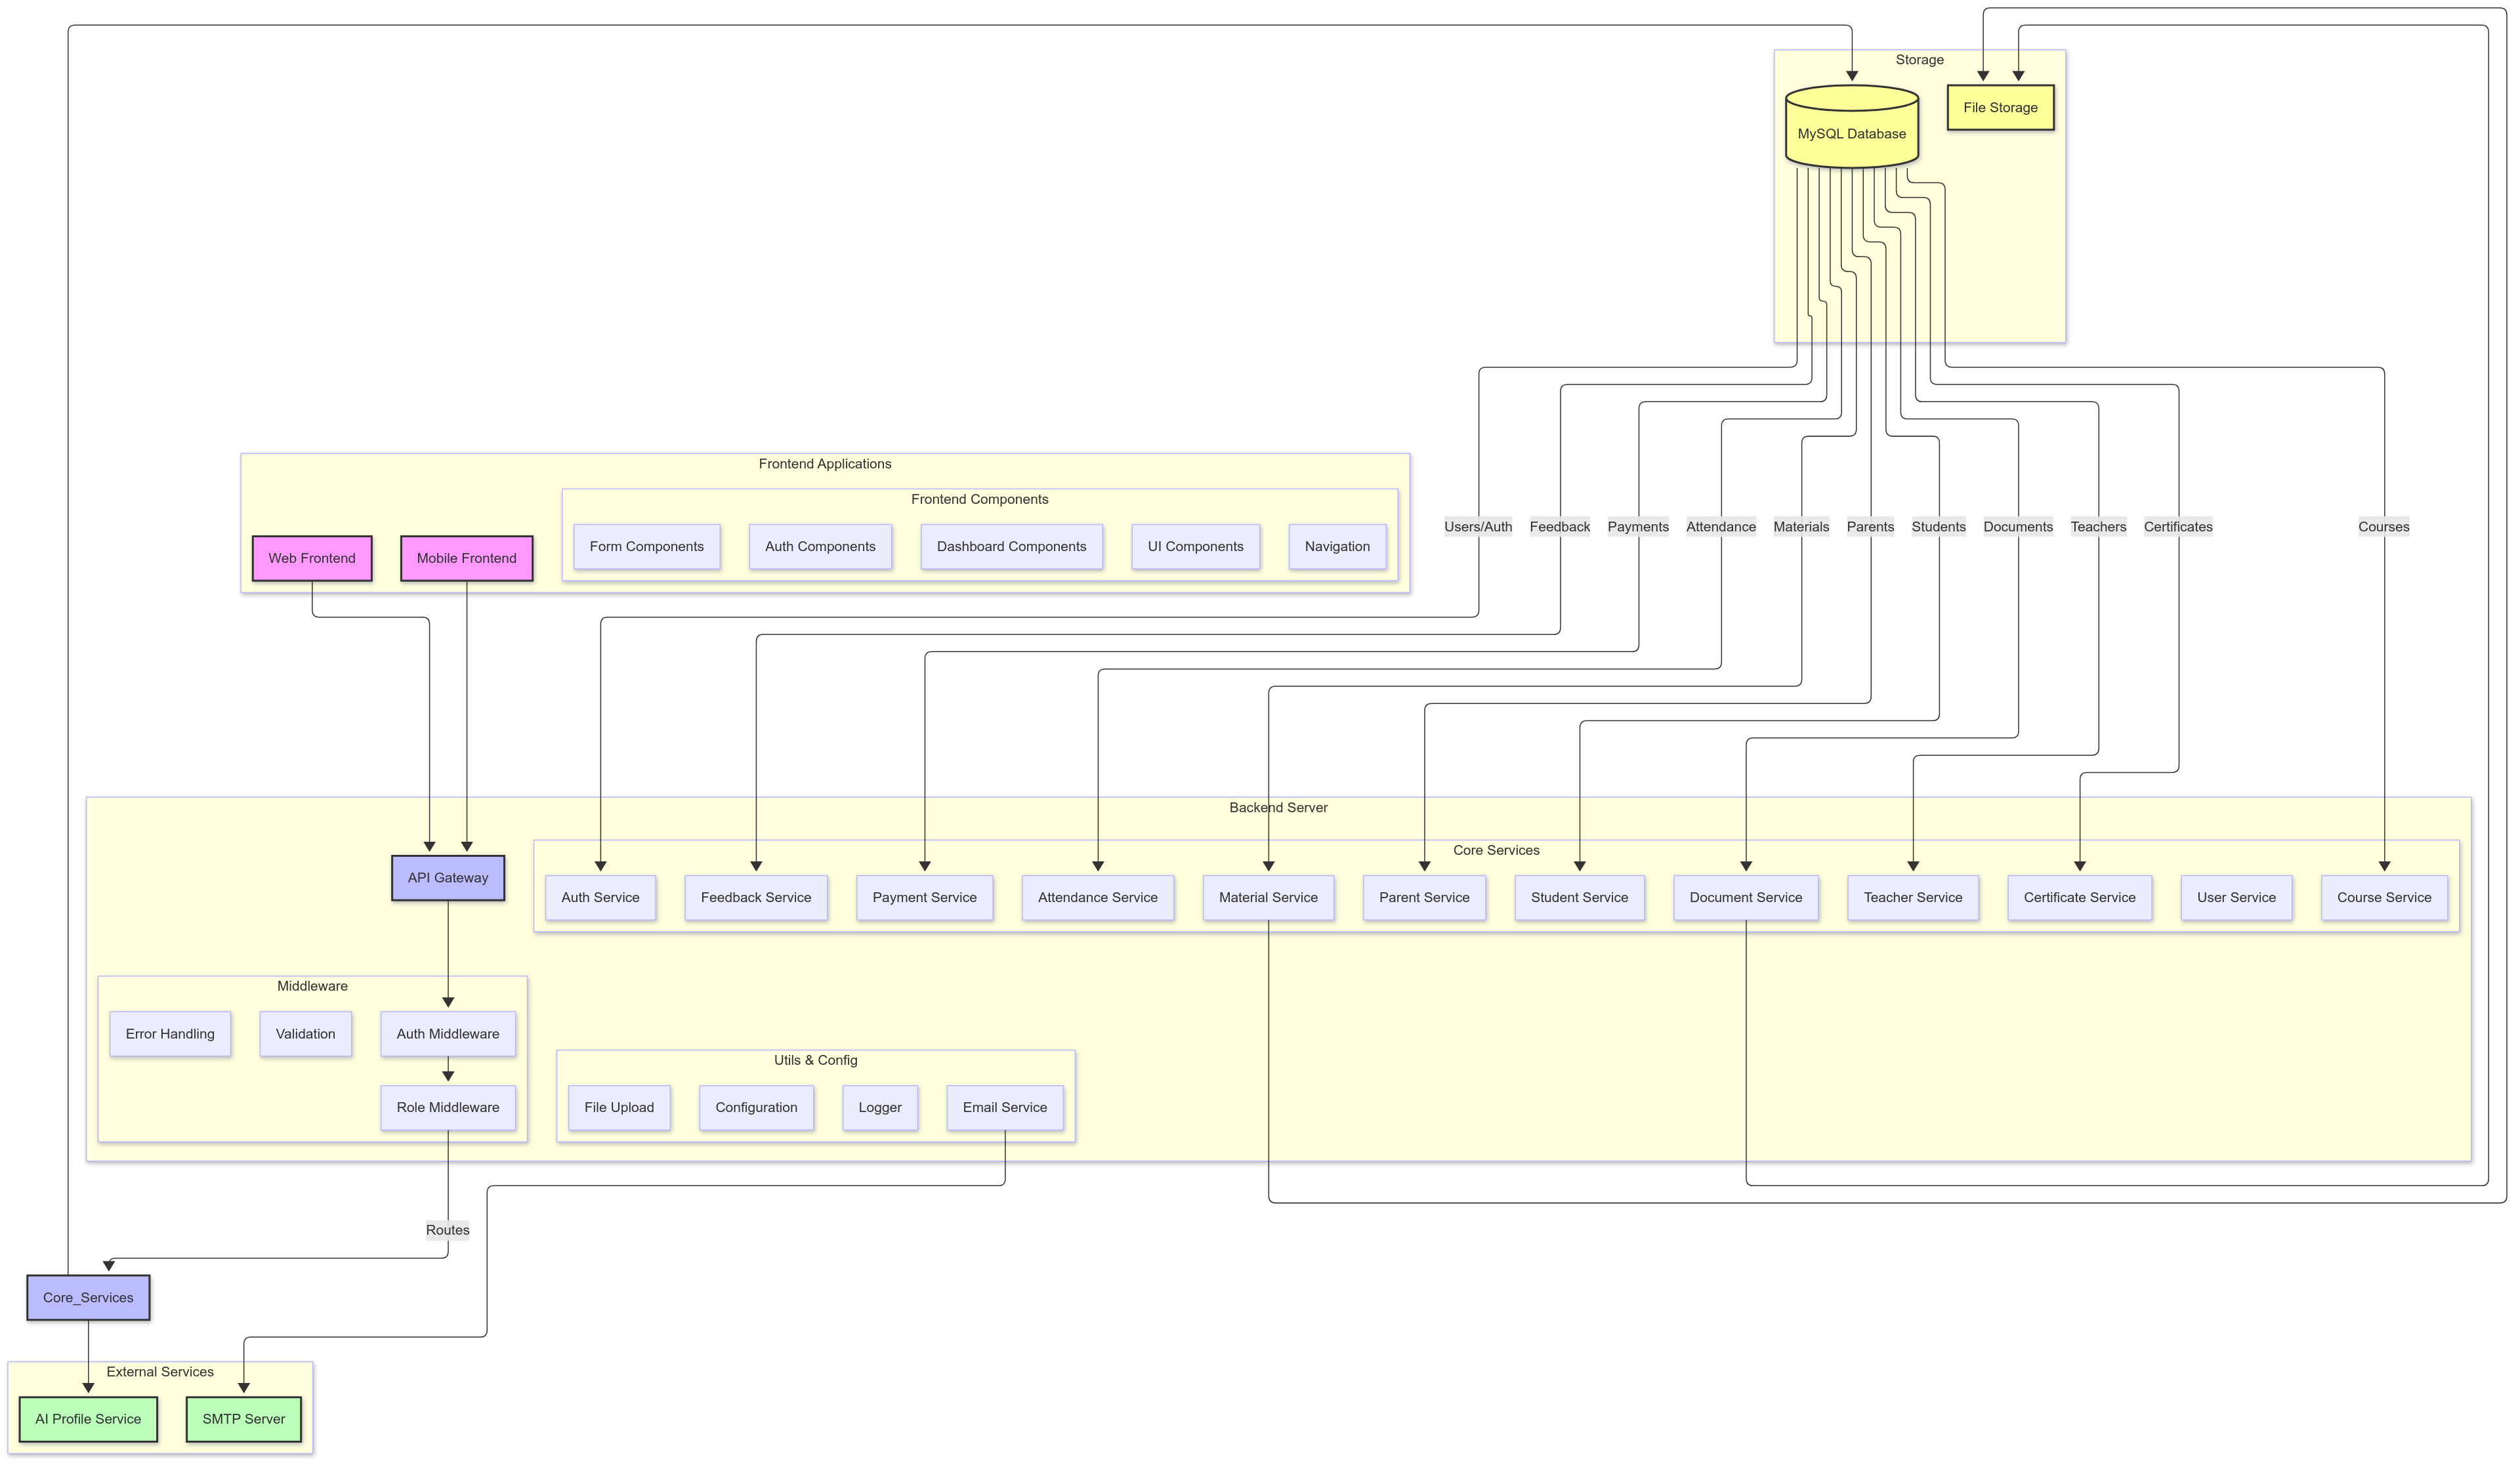
\includegraphics[width=\textwidth,height=0.6\textheight,keepaspectratio]{../pfe-pics/diagrames/archetecture.png}
            \caption{System Architecture Overview}
        \end{figure}
    \end{columns}
\end{frame}

\begin{frame}{Objectives}
    \begin{itemize}
        \item \textbf{School Management System}
        \begin{itemize}
            \item Centralize and streamline academic processes
            \item Enable real-time communication between stakeholders
            \item Simplify administrative tasks
            \item Provide intuitive interfaces for all user types
        \end{itemize}
        \vspace{0.5cm}
        \item \textbf{AI Profiles Creation}
        \begin{itemize}
            \item Transform educational materials into interactive AI profiles
            \item Create personalized learning experiences
            \item Enhance course understanding through AI-assisted explanations
            \item Integrate AI profiles with the school management platform
        \end{itemize}
    \end{itemize}
\end{frame}

\section{System Architecture}

\begin{frame}{Global Architecture}
    \begin{columns}
        \column{0.5\textwidth}
        \textbf{Multi-layered approach:}
        \begin{itemize}
            \item Presentation Layer
            \item API Layer
            \item Business Layer
            \item Persistence Layer
            \item Cross-cutting Services
        \end{itemize}
        \column{0.5\textwidth}
        \begin{figure}
            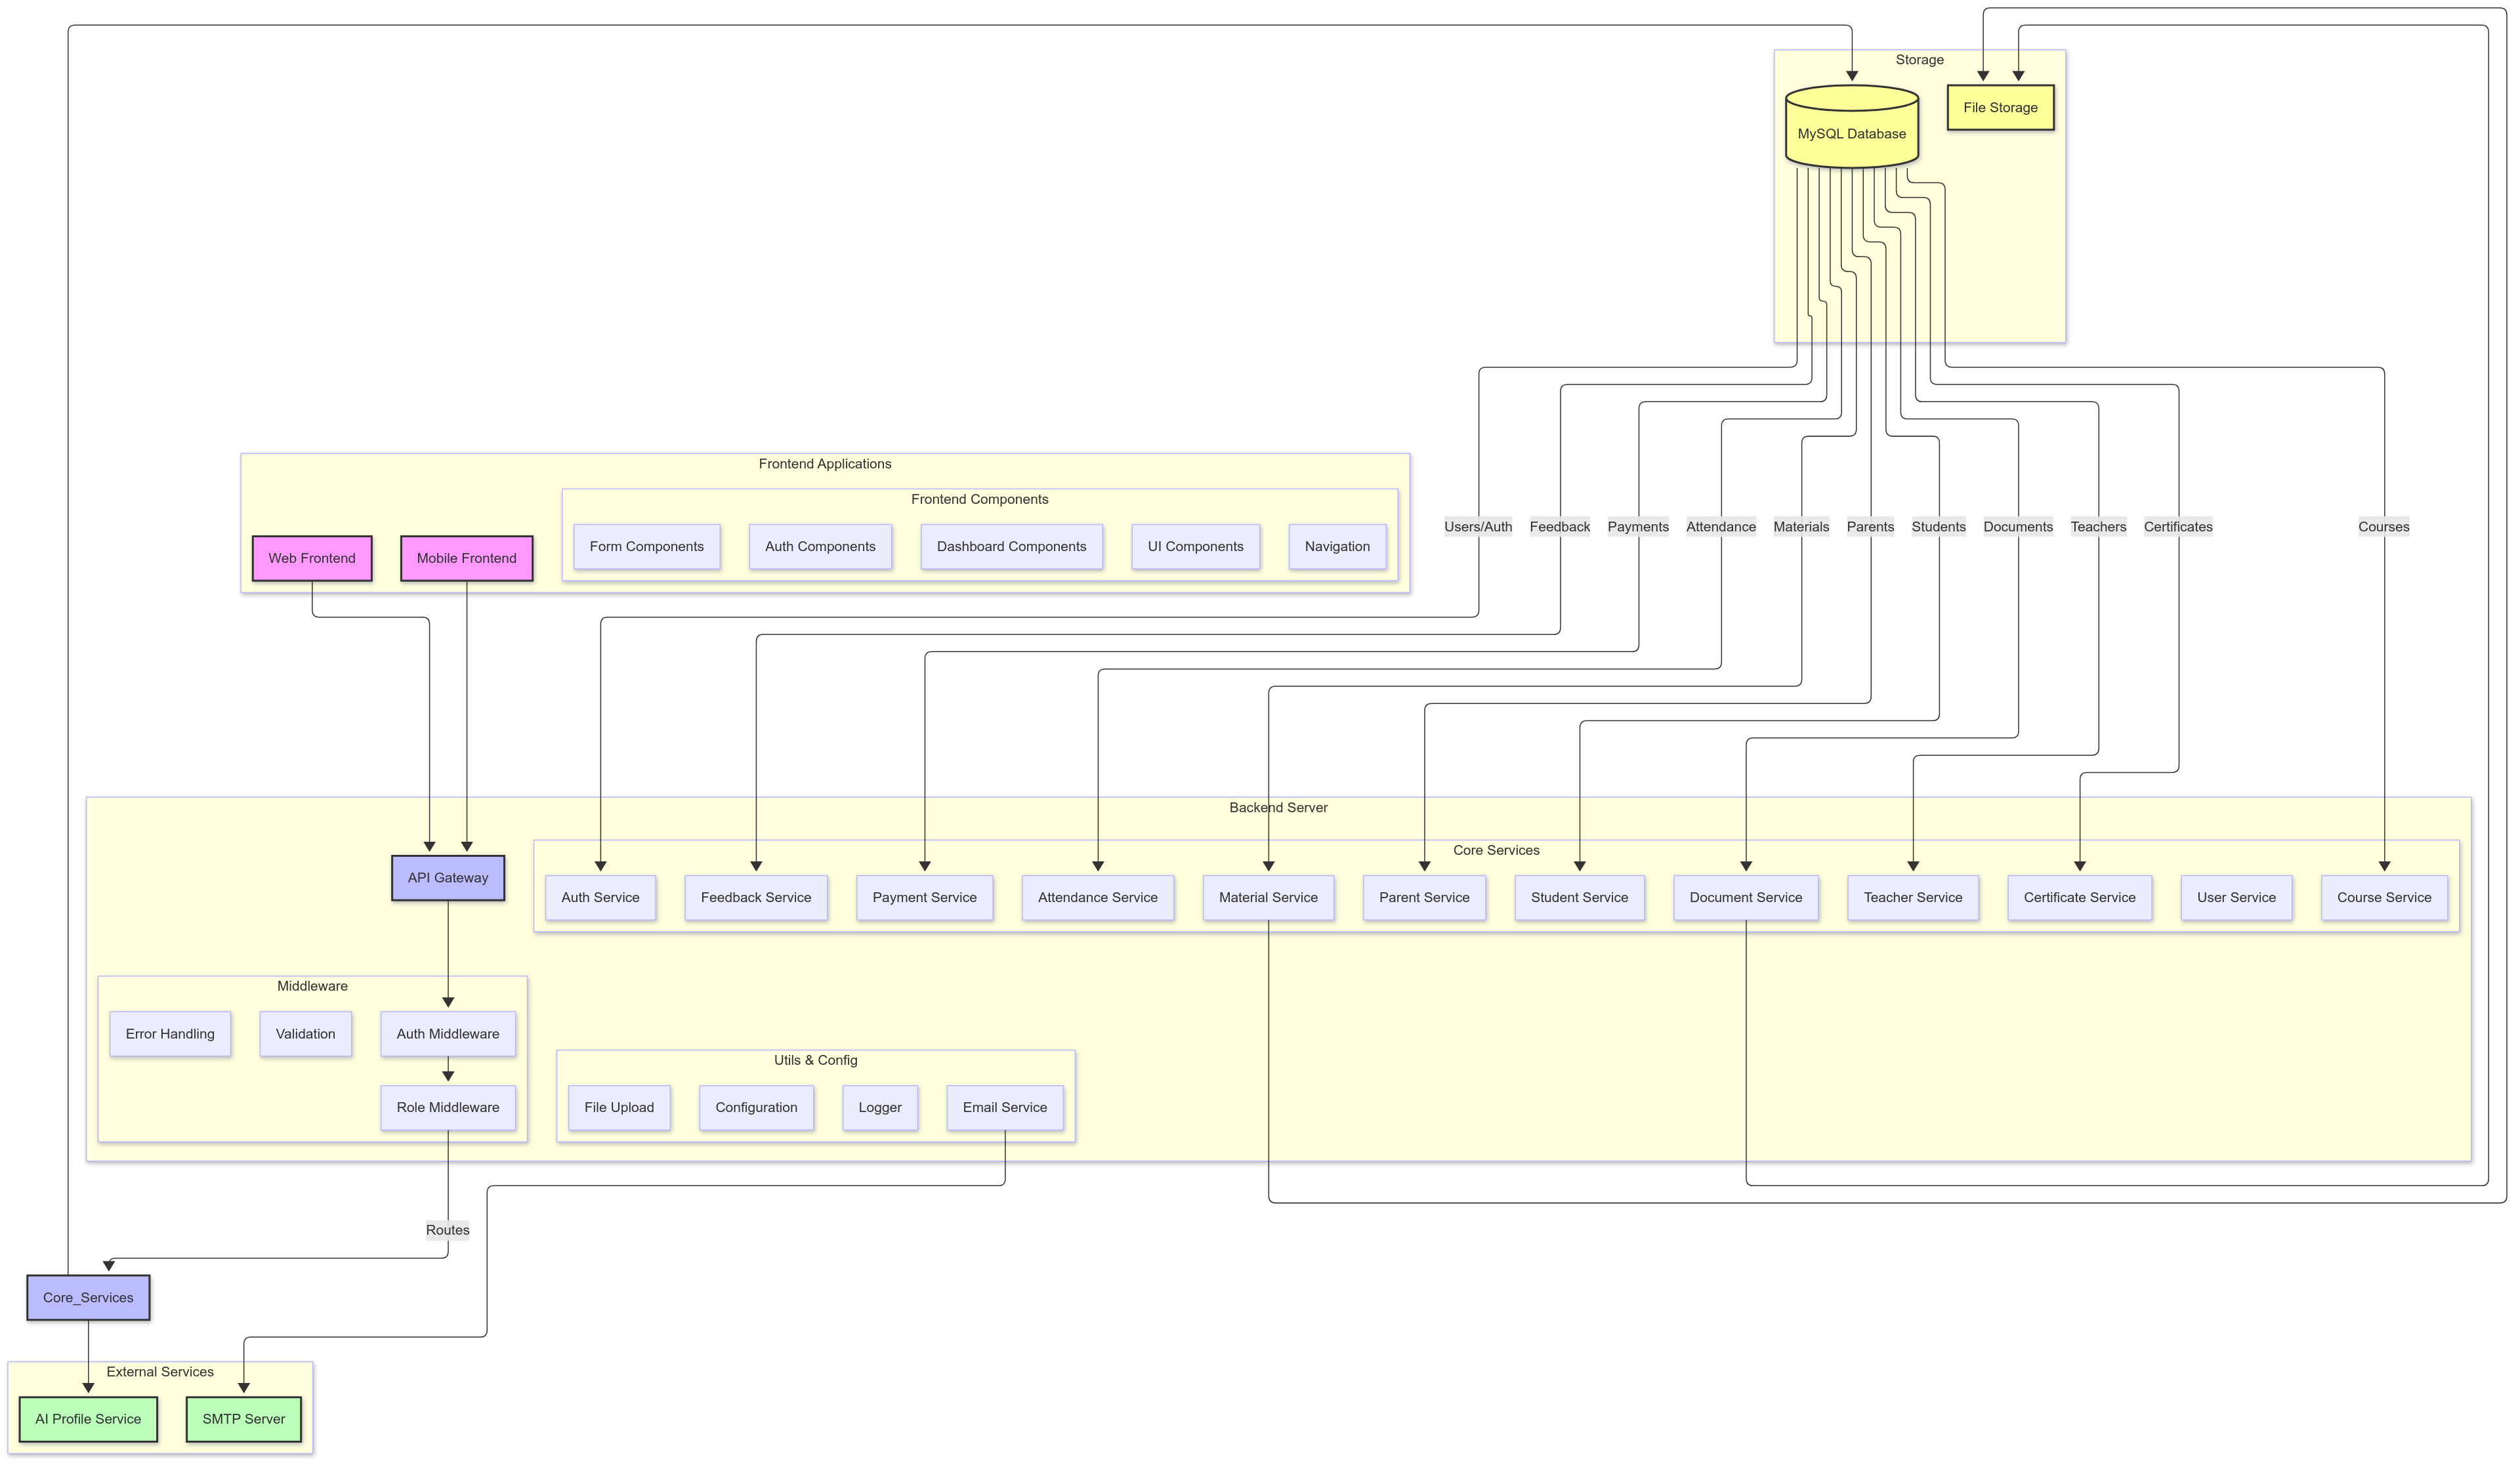
\includegraphics[width=\textwidth,height=0.6\textheight,keepaspectratio]{../pfe-pics/diagrames/archetecture.png}
            \caption{Layered Architecture Diagram}
        \end{figure}
    \end{columns}
\end{frame}

\begin{frame}{School Management System Architecture}
    \begin{columns}
        \column{0.6\textwidth}
        \textbf{Frontend:}
        \begin{itemize}
            \item React with TypeScript (Web)
            \item React Native (Mobile)
            \item Tailwind CSS for styling
        \end{itemize}
        \textbf{Backend:}
        \begin{itemize}
            \item RESTful API architecture
            \item Express.js server
            \item MongoDB database
            \item JWT authentication
        \end{itemize}
        \column{0.4\textwidth}
        \begin{figure}
            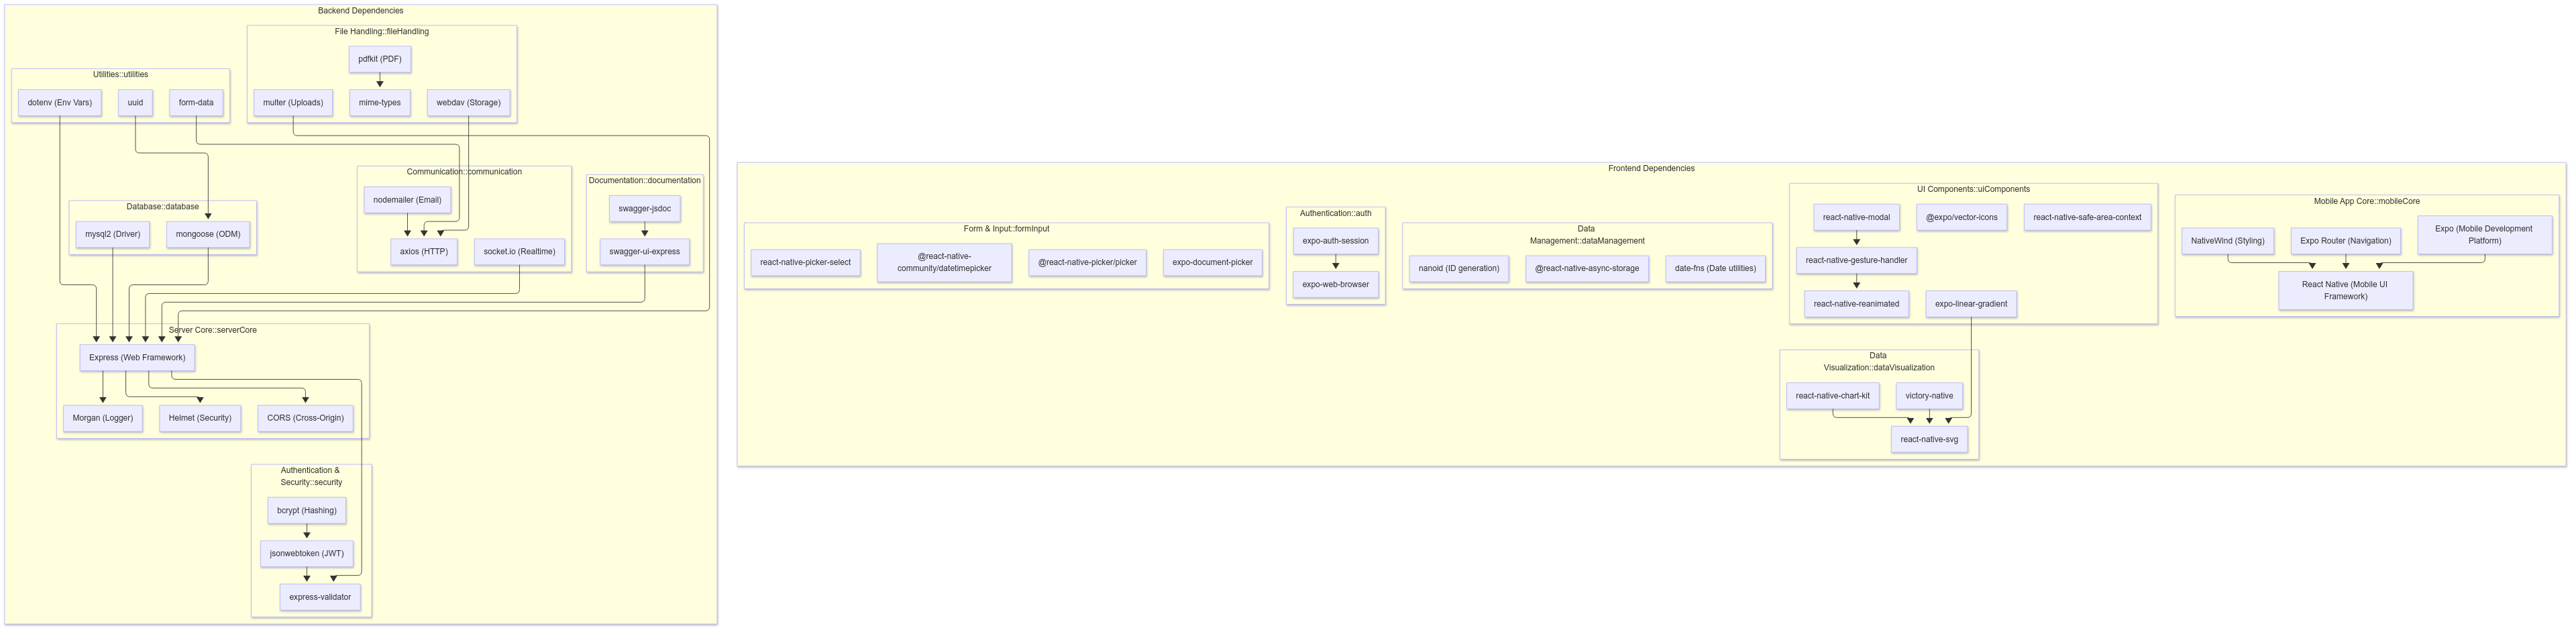
\includegraphics[width=\textwidth,height=0.6\textheight,keepaspectratio]{../pfe-pics/diagrames/dependeces.png}
            \caption{System Dependencies}
        \end{figure}
    \end{columns}
\end{frame}

\begin{frame}{AI Profiles Creation Architecture}
    \begin{columns}
        \column{0.55\textwidth}
        \textbf{Components:}
        \begin{itemize}
            \item Profile Manager
            \item Document Processor
            \item Indexing Engine
            \item Conversational Interface
            \item API Gateway
            \item Authentication System
        \end{itemize}
        \column{0.45\textwidth}
        \begin{figure}
            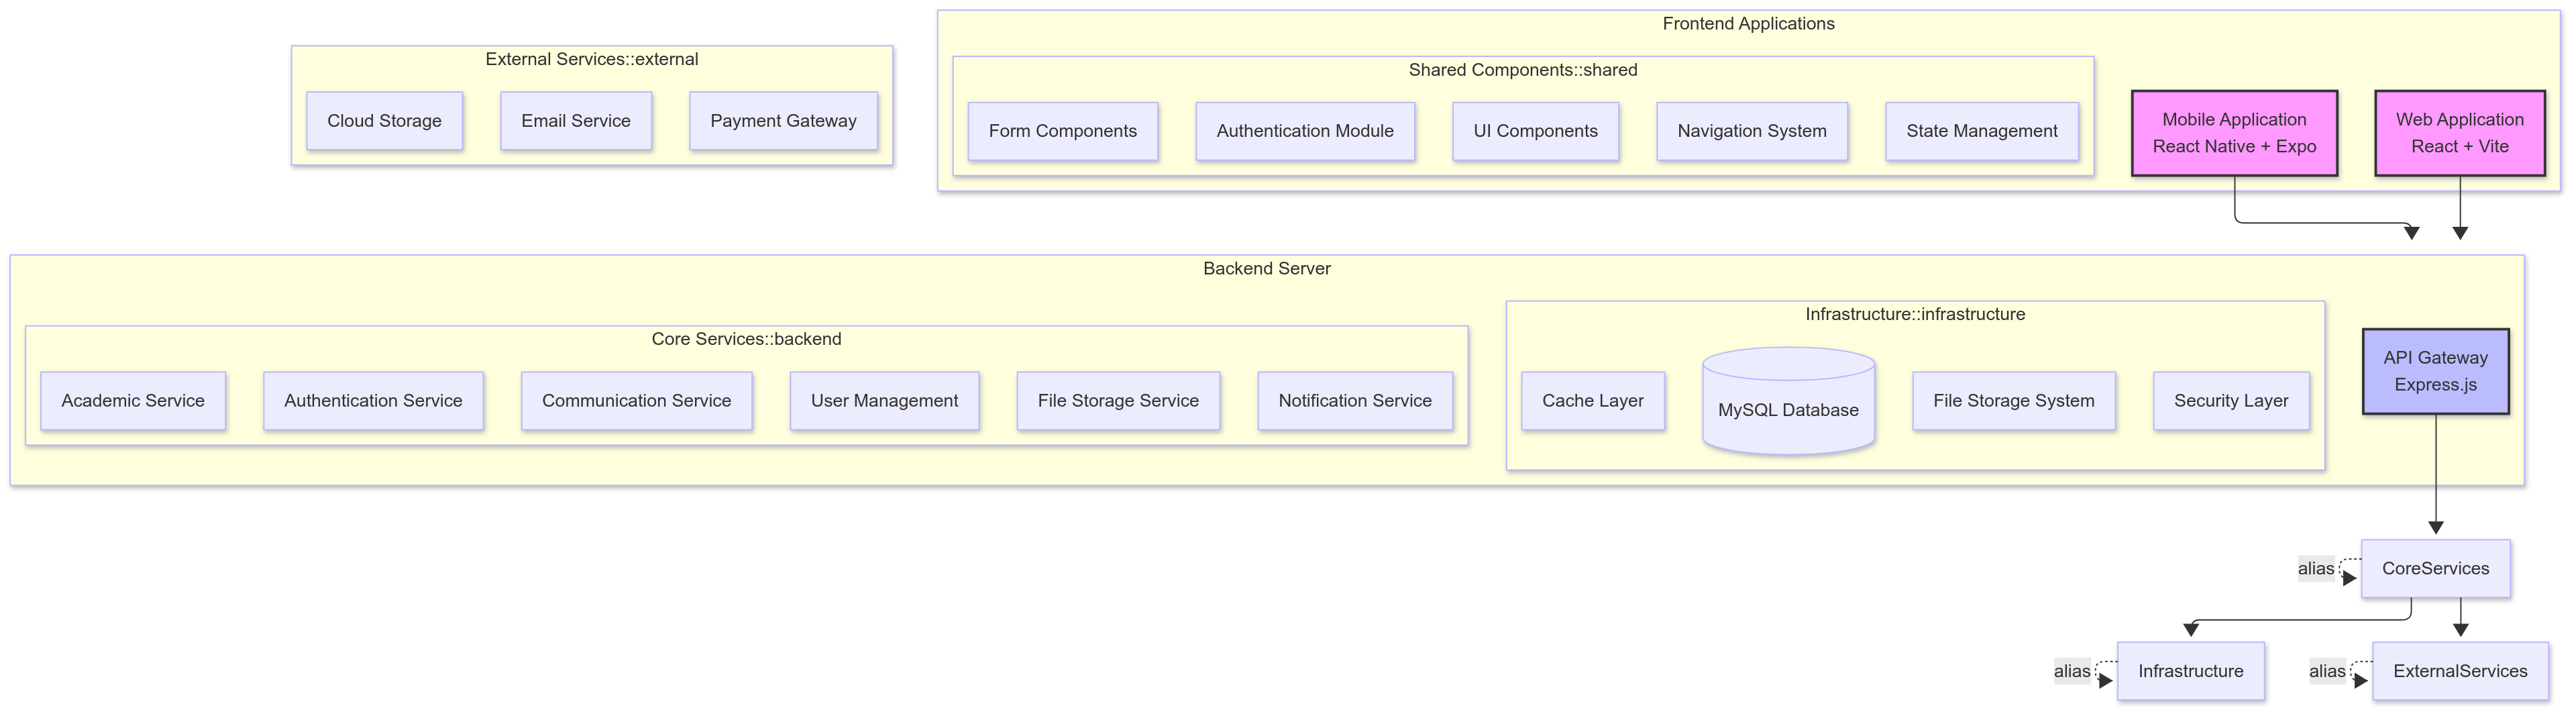
\includegraphics[width=\textwidth,height=0.6\textheight,keepaspectratio]{../pfe-pics/diagrames/Component Diagram (showing the system_s architecture).png}
            \caption{Component Architecture}
        \end{figure}
    \end{columns}
\end{frame}

\begin{frame}{Data Model}
    \begin{figure}
        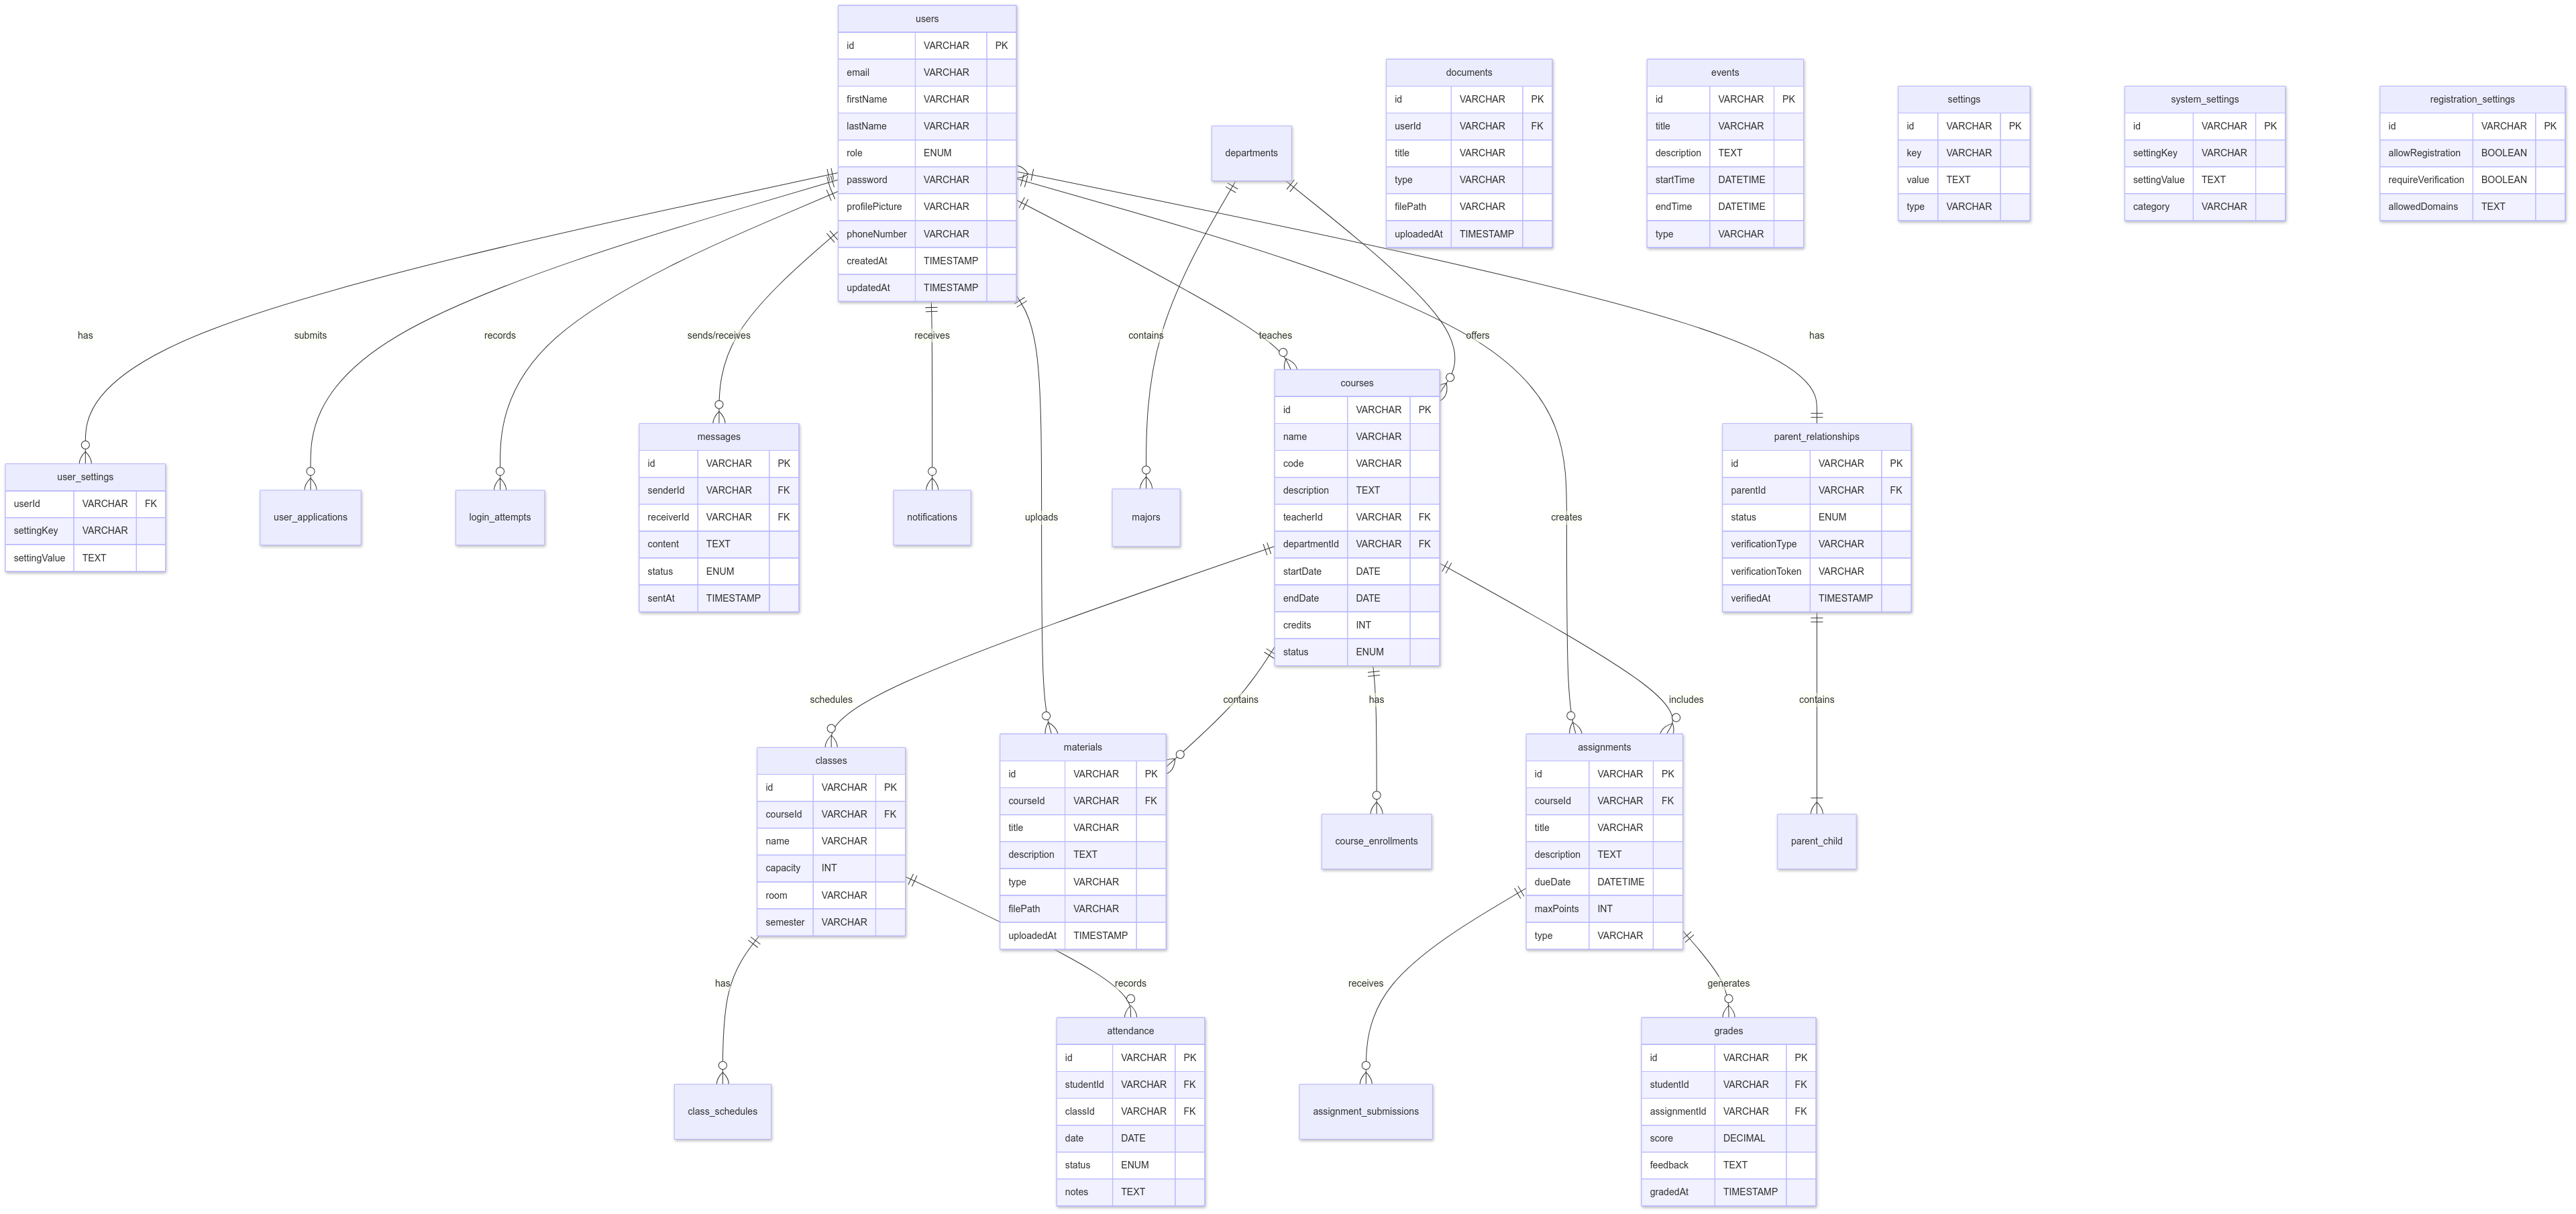
\includegraphics[width=0.85\textwidth,height=0.7\textheight,keepaspectratio]{../pfe-pics/diagrames/tabaales.png}
        \caption{Entity Relationship Diagram}
    \end{figure}
    \begin{itemize}
        \item Comprehensive entity relationships
        \item User roles with appropriate permissions
        \item Course management structures
        \item Assessment and grading systems
    \end{itemize}
\end{frame}

\section{Key Features}

\begin{frame}{School Management System Features}
    \begin{columns}
        \column{0.5\textwidth}
        \textbf{For Administrators:}
        \begin{itemize}
            \item User management
            \item Course creation
            \item Teacher assignment
            \item Analytics dashboard
        \end{itemize}
        \textbf{For Teachers:}
        \begin{itemize}
            \item Course material uploads
            \item Attendance tracking
            \item Assignment creation
            \item Grade management
        \end{itemize}
        \column{0.5\textwidth}
        \textbf{For Students:}
        \begin{itemize}
            \item Course enrollment
            \item Assignment submission
            \item Performance tracking
            \item Communication tools
        \end{itemize}
        \textbf{For Parents:}
        \begin{itemize}
            \item Child progress monitoring
            \item Teacher communication
            \item Attendance notifications
            \item Event calendar
        \end{itemize}
    \end{columns}
\end{frame}

\begin{frame}{AI Profiles Creation Features}
    \begin{columns}
        \column{0.5\textwidth}
        \textbf{Document Processing:}
        \begin{itemize}
            \item Multi-format support
            \item Text extraction
            \item Structural analysis
            \item Semantic enrichment
        \end{itemize}
        \textbf{Knowledge Management:}
        \begin{itemize}
            \item Intelligent chunking
            \item Vector embeddings
            \item Metadata organization
            \item Version control
        \end{itemize}
        \column{0.5\textwidth}
        \textbf{AI Interaction:}
        \begin{itemize}
            \item Context-aware responses
            \item Source attribution
            \item Conversation history
            \item Query optimization
        \end{itemize}
        \textbf{Integration:}
        \begin{itemize}
            \item API access
            \item Course embedding
            \item Permission management
            \item Usage analytics
        \end{itemize}
    \end{columns}
\end{frame}

\begin{frame}{Landing Page - Hero Section}
    \begin{figure}
        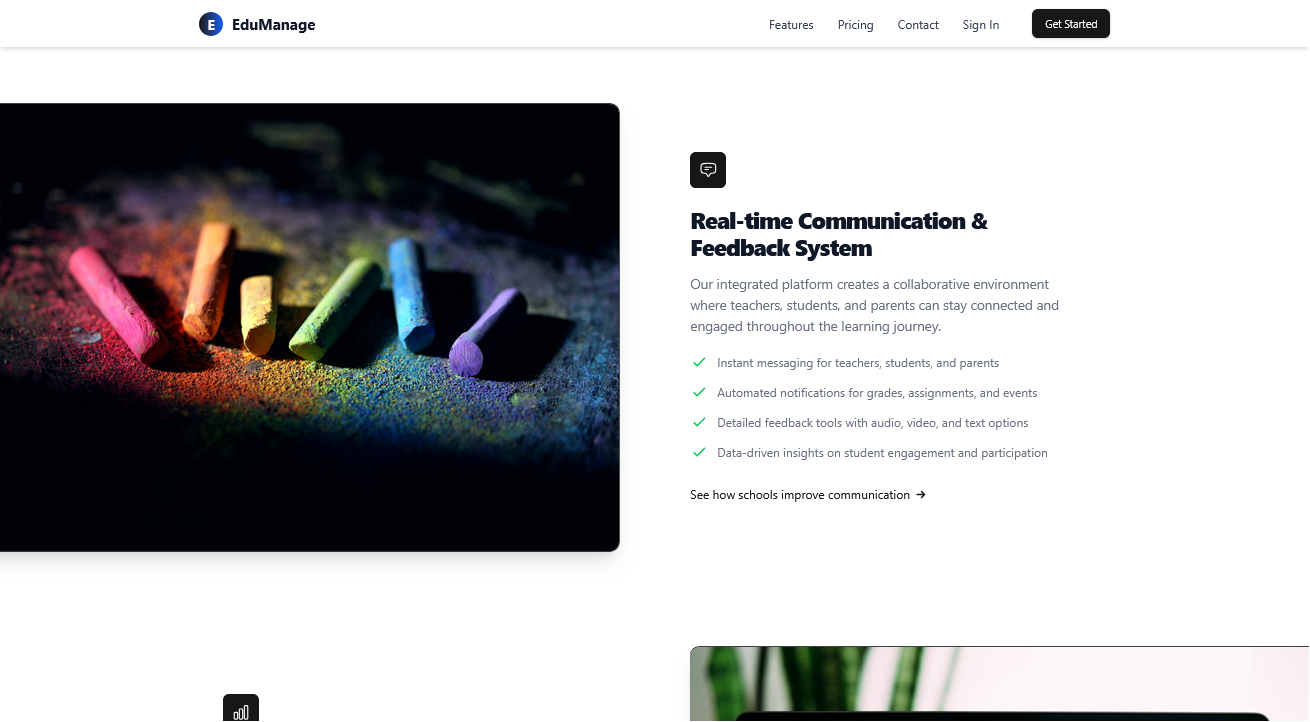
\includegraphics[width=0.9\textwidth,height=0.7\textheight,keepaspectratio]{../pfe-pics/landing/Screenshot 2025-06-09 at 23-12-17 Vite React TS.png}
        \caption{Main landing page with key value proposition and call-to-action}
    \end{figure}
\end{frame}

\begin{frame}{Landing Page - Feature Highlights}
    \begin{columns}
        \column{0.5\textwidth}
        \begin{figure}
            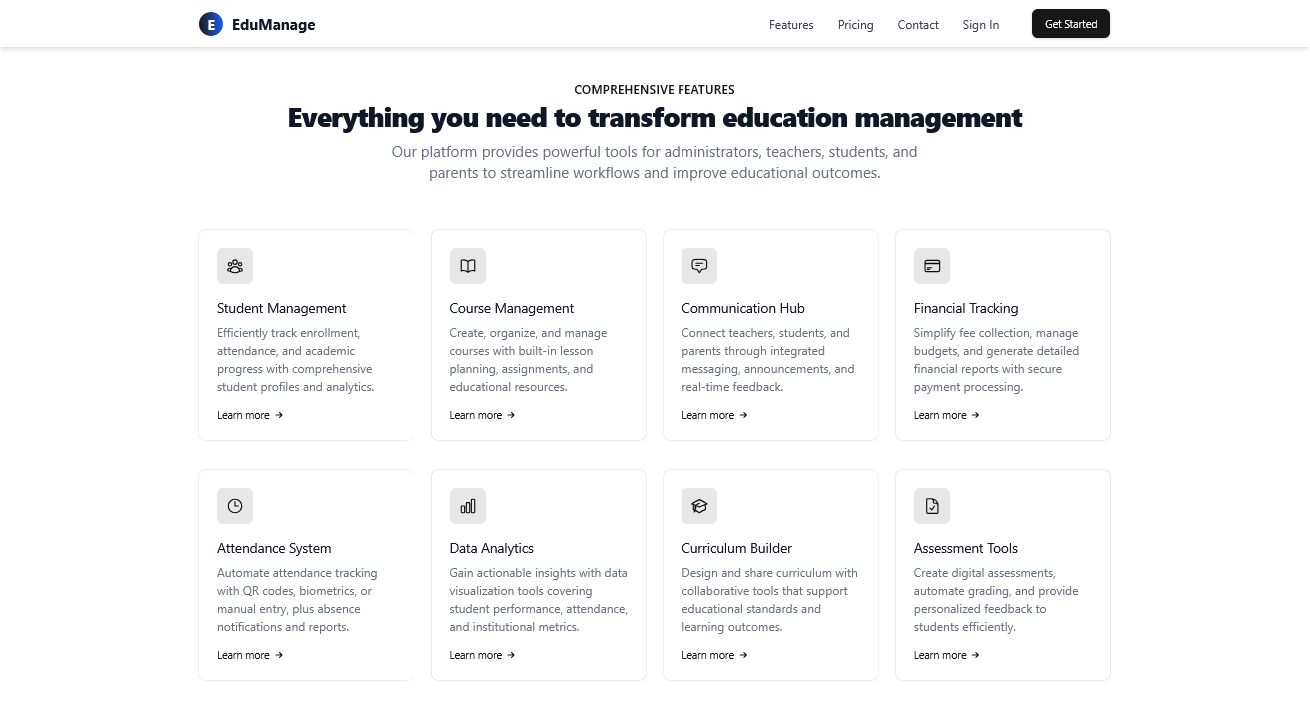
\includegraphics[width=\textwidth,height=0.6\textheight,keepaspectratio]{../pfe-pics/landing/info.png}
            \caption{Key features highlight section}
        \end{figure}
        \column{0.5\textwidth}
        \begin{figure}
            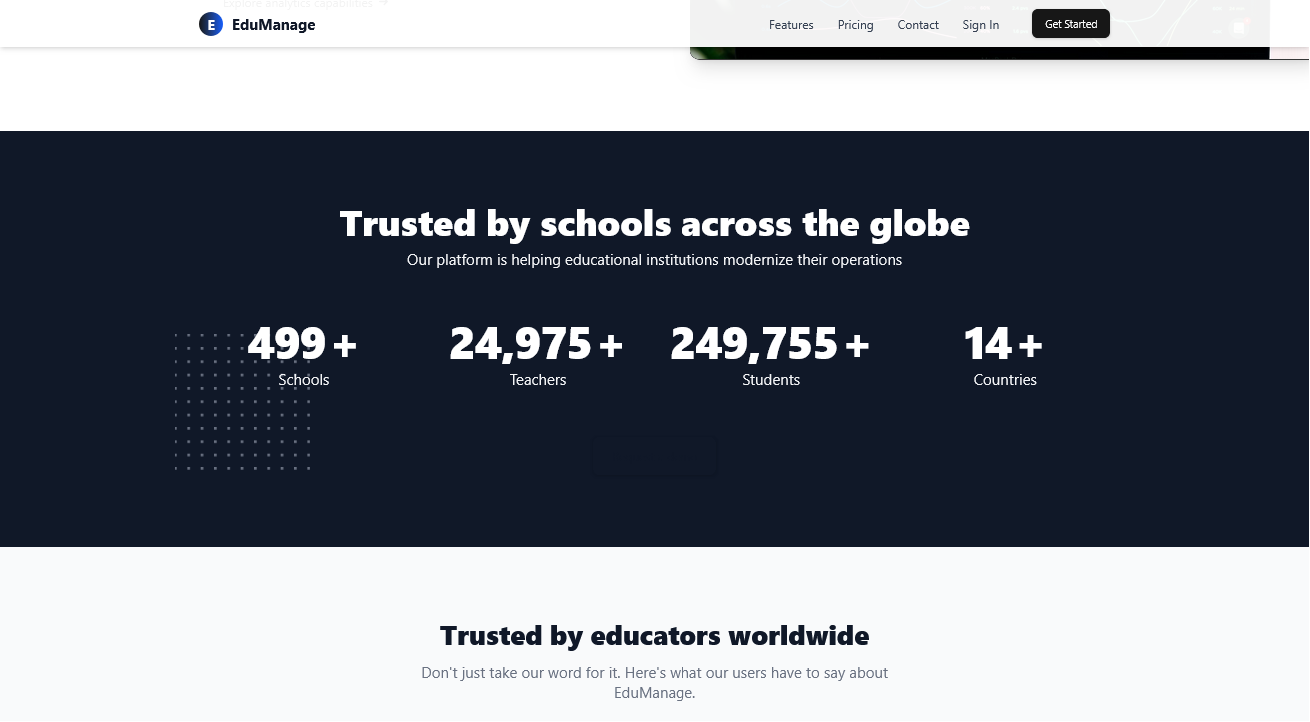
\includegraphics[width=\textwidth,height=0.6\textheight,keepaspectratio]{../pfe-pics/landing/stats.png}
            \caption{Platform statistics section}
        \end{figure}
    \end{columns}
\end{frame}

\begin{frame}{Authentication Flow}
    \begin{columns}
        \column{0.5\textwidth}
        \begin{figure}
            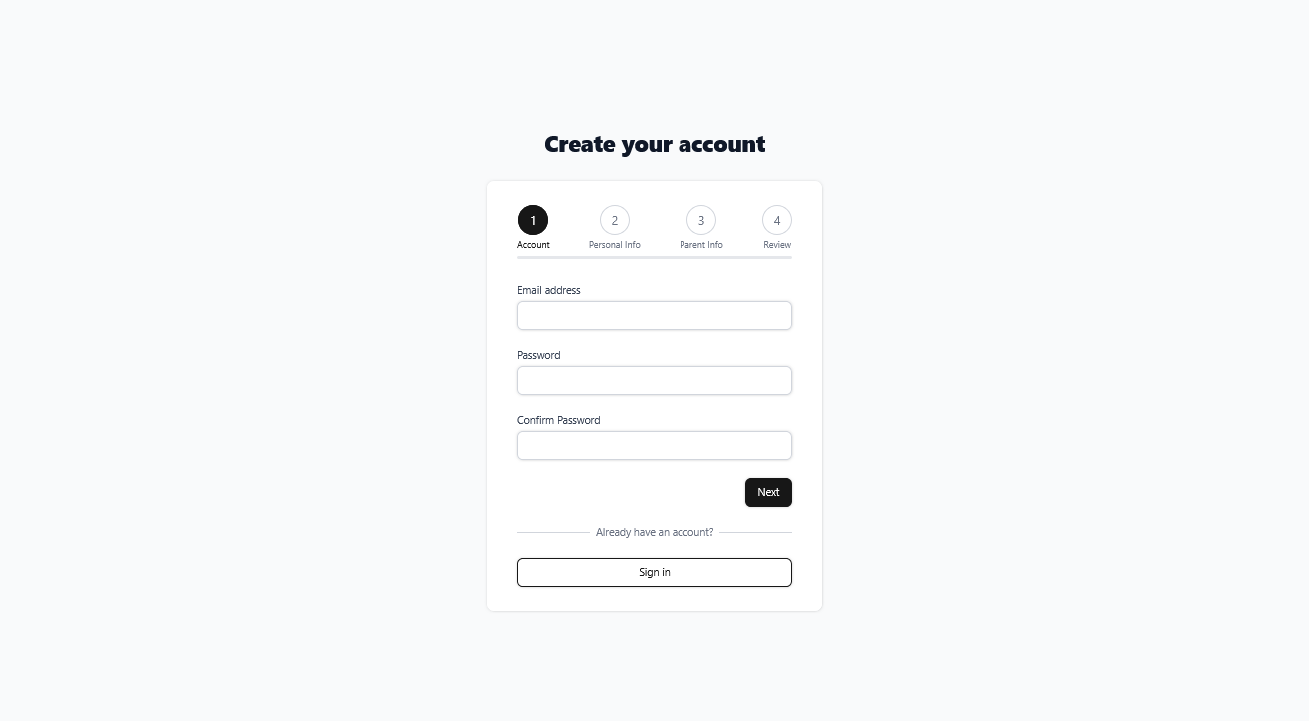
\includegraphics[width=\textwidth,height=0.6\textheight,keepaspectratio]{../pfe-pics/auth/Screenshot 2025-06-09 at 23-00-18 Vite React TS.png}
            \caption{Login interface}
        \end{figure}
        \column{0.5\textwidth}
        \begin{figure}
            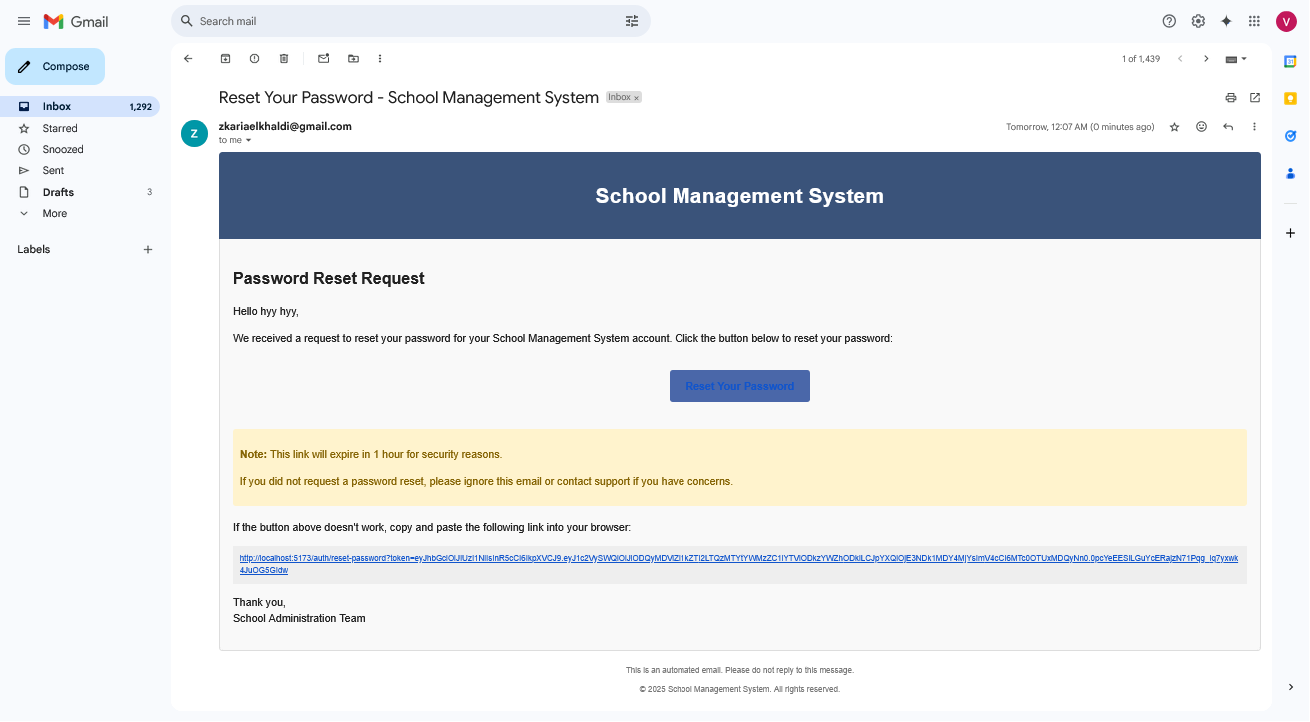
\includegraphics[width=\textwidth,height=0.6\textheight,keepaspectratio]{../pfe-pics/auth/Screenshot 2025-06-09 at 23-08-41 Reset Your Password - School Management System - vertigoevilman1@gmail.com - Gmail.png}
            \caption{Password reset workflow}
        \end{figure}
    \end{columns}
\end{frame}

\begin{frame}{Web Interface - Administrator Dashboard}
    \begin{figure}
        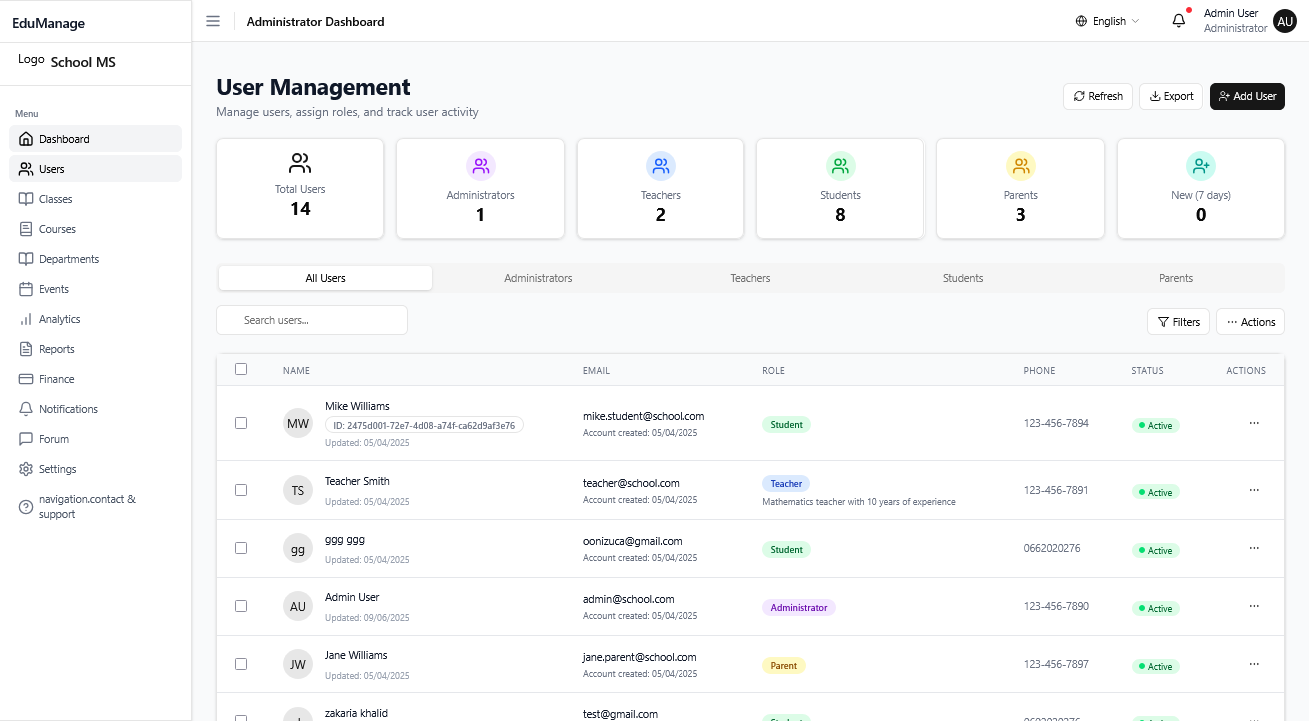
\includegraphics[width=0.9\textwidth,height=0.6\textheight,keepaspectratio]{../pfe-pics/admin/Screenshot 2025-06-09 at 22-38-38 Vite React TS.png}
        \caption{Admin analytics dashboard with key performance indicators}
    \end{figure}
\end{frame}

\begin{frame}{Web Interface - Administrator Tools}
    \begin{columns}
        \column{0.5\textwidth}
        \begin{figure}
            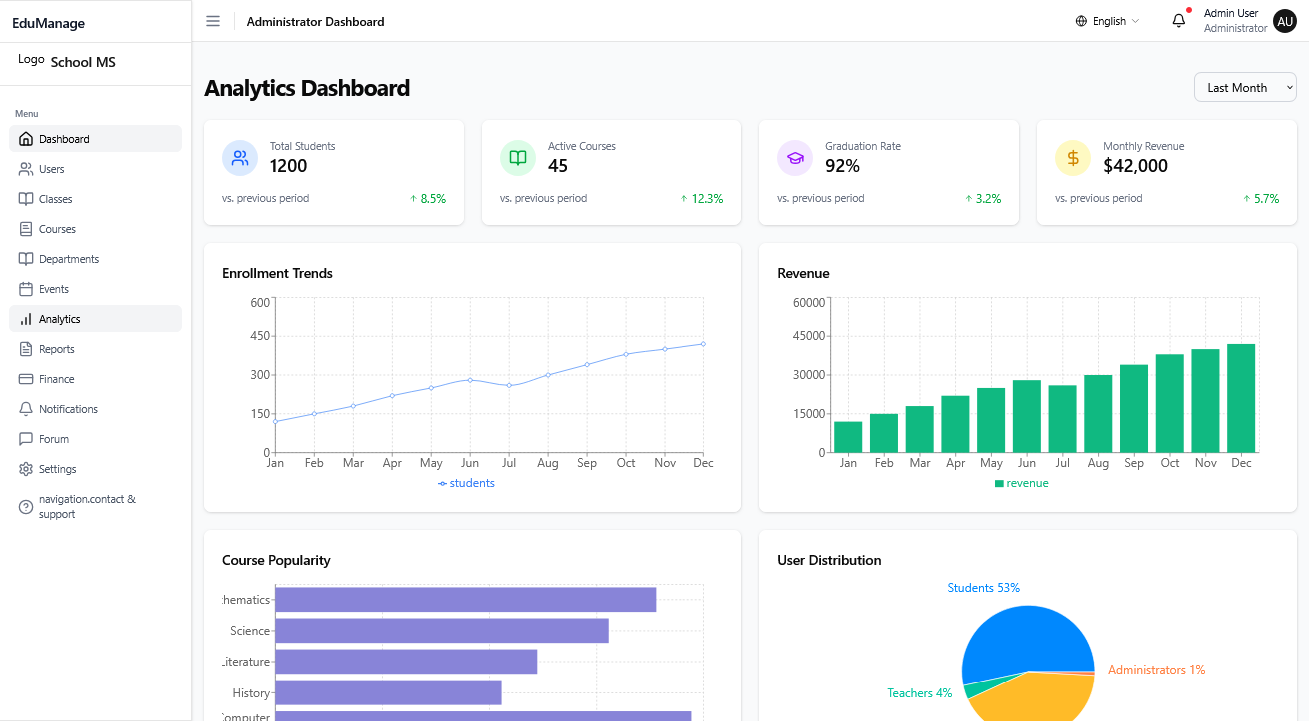
\includegraphics[width=\textwidth,height=0.55\textheight,keepaspectratio]{../pfe-pics/admin/Screenshot 2025-06-09 at 22-40-11 Vite React TS.png}
            \caption{User management interface}
        \end{figure}
        \column{0.5\textwidth}
        \begin{figure}
            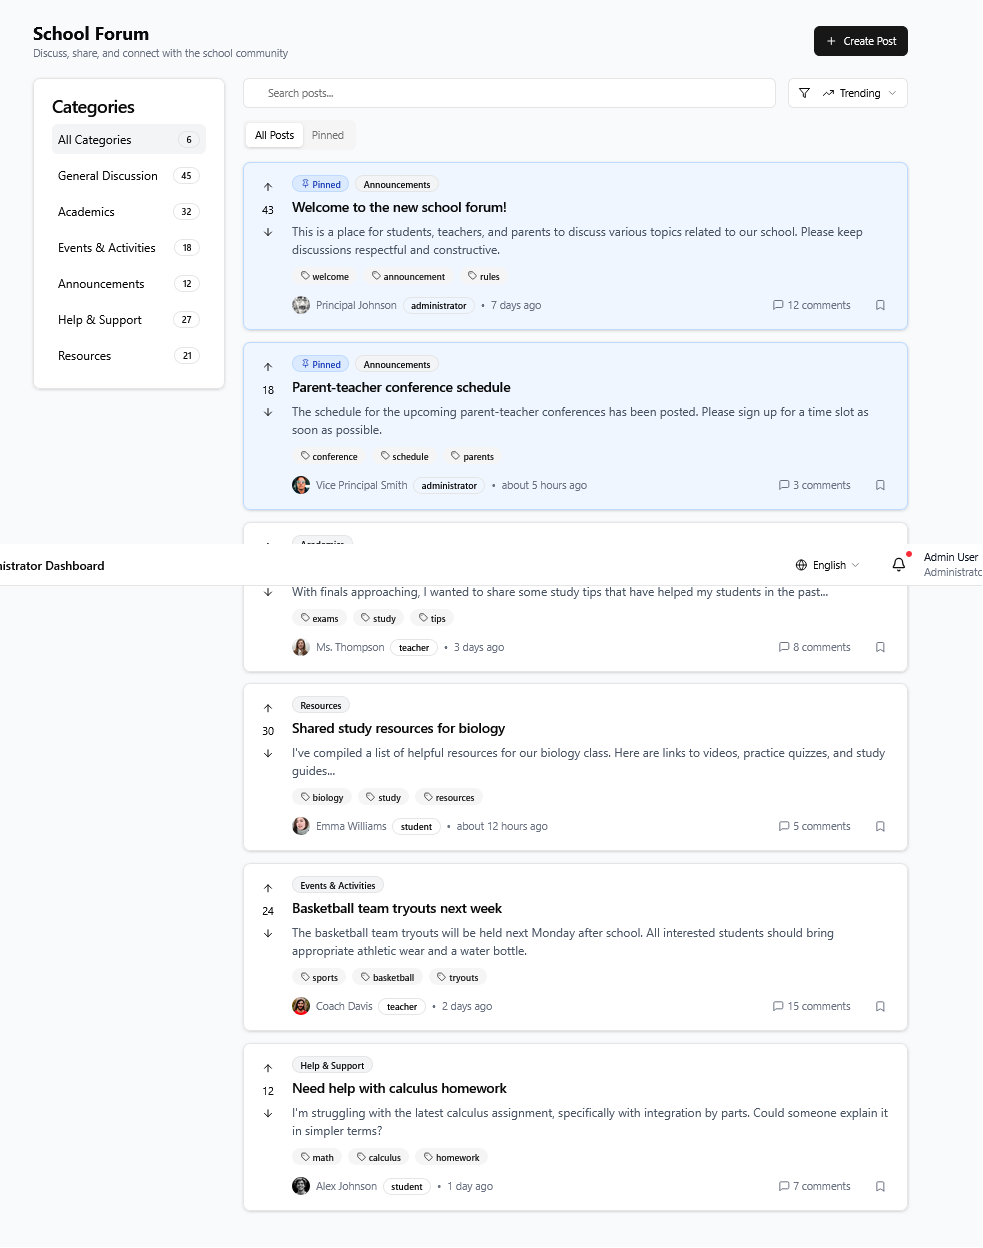
\includegraphics[width=\textwidth,height=0.55\textheight,keepaspectratio]{../pfe-pics/admin/Screenshot 2025-06-09 at 22-41-16 Vite React TS.png}
            \caption{System configuration panel}
        \end{figure}
    \end{columns}
\end{frame}

\begin{frame}{Web Interface - Teacher Tools}
    \begin{columns}
        \column{0.5\textwidth}
        \begin{figure}
            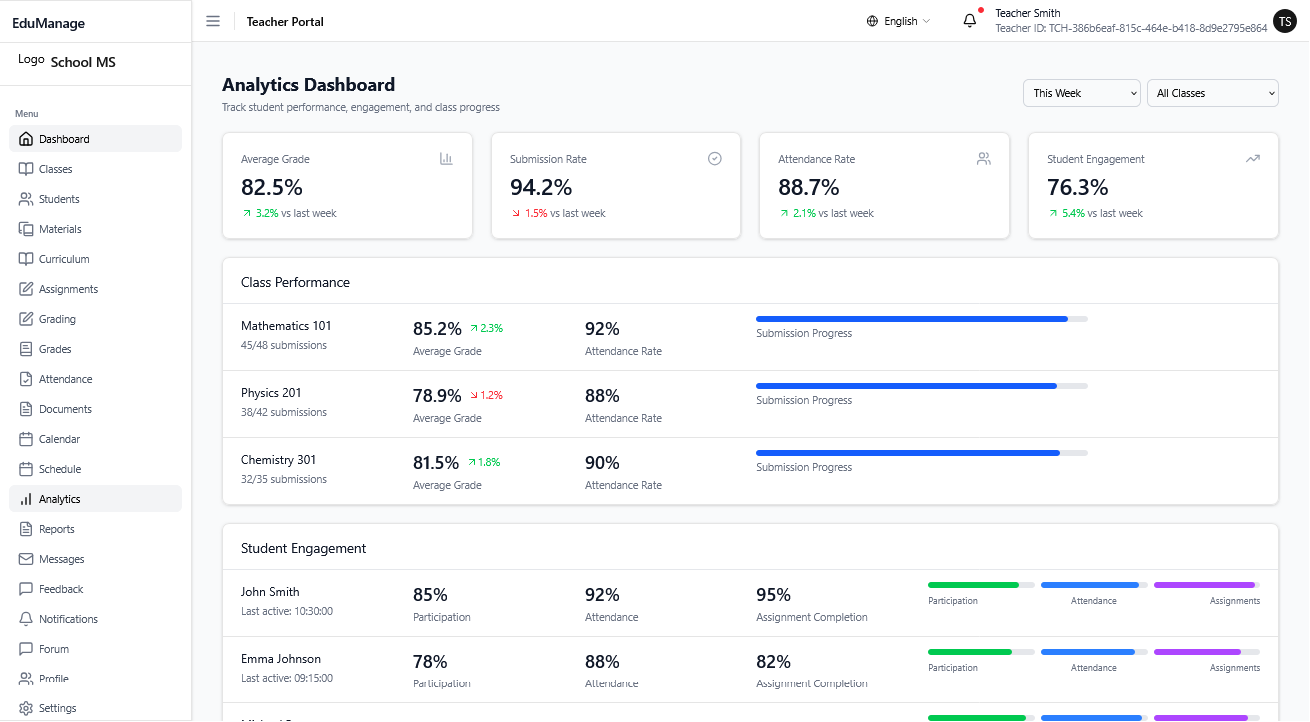
\includegraphics[width=\textwidth,height=0.55\textheight,keepaspectratio]{../pfe-pics/teacher/Screenshot 2025-06-09 at 22-55-38 Vite React TS.png}
            \caption{Course management interface}
        \end{figure}
        \column{0.5\textwidth}
        \begin{figure}
            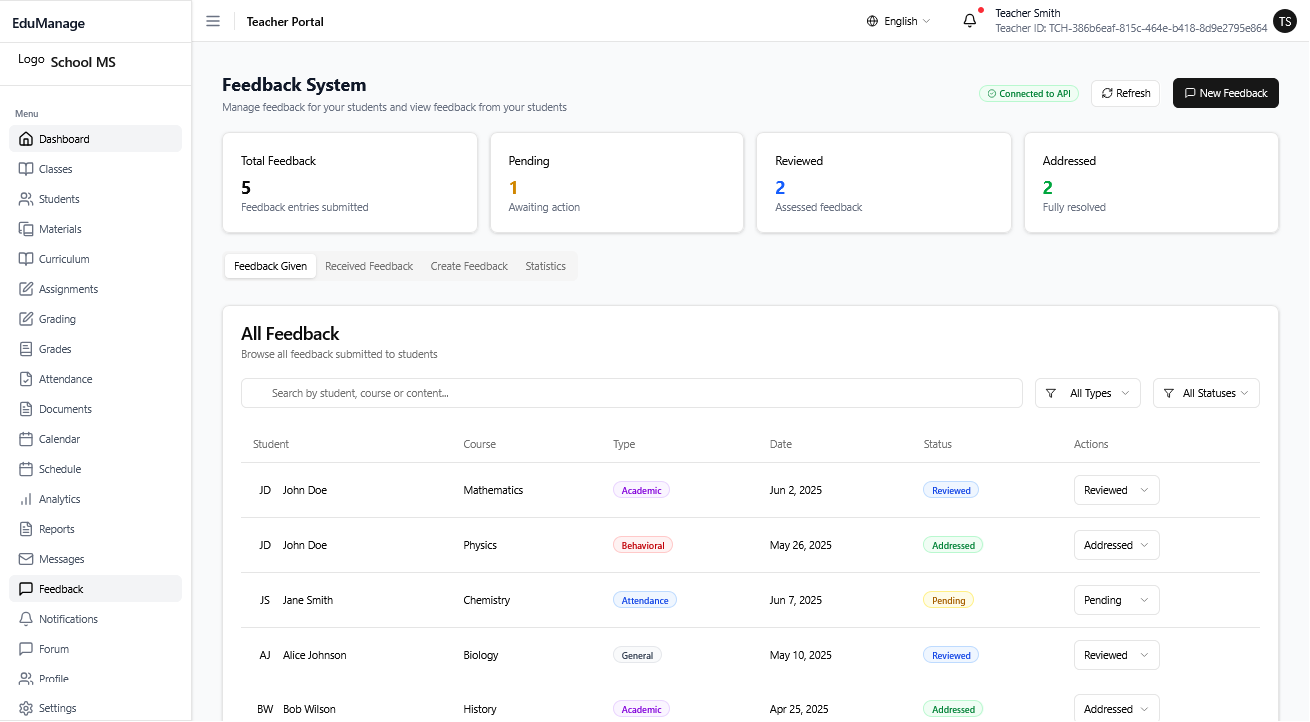
\includegraphics[width=\textwidth,height=0.55\textheight,keepaspectratio]{../pfe-pics/teacher/Screenshot 2025-06-09 at 22-56-28 Vite React TS.png}
            \caption{Student grading system}
        \end{figure}
    \end{columns}
\end{frame}

\begin{frame}{Web Interface - Student View}
    \begin{columns}
        \column{0.5\textwidth}
        \begin{figure}
            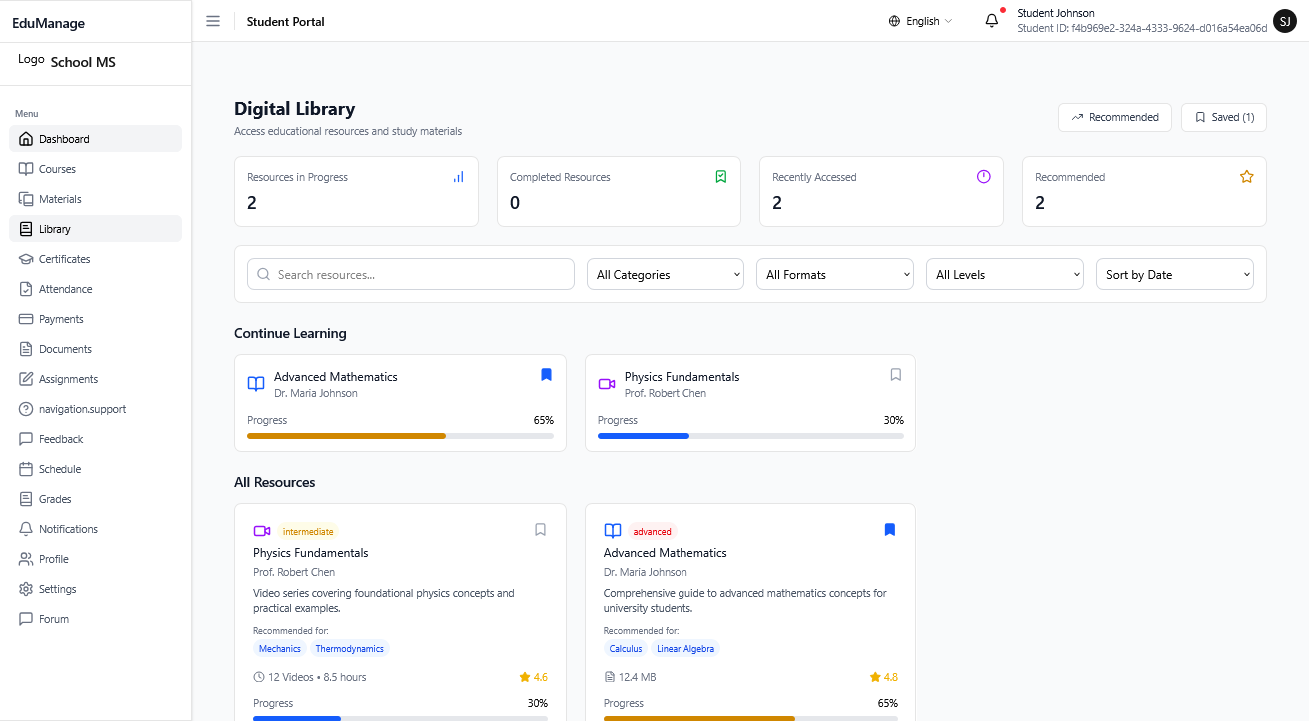
\includegraphics[width=\textwidth,height=0.55\textheight,keepaspectratio]{../pfe-pics/student/Screenshot 2025-06-09 at 22-45-09 Vite React TS.png}
            \caption{Course enrollment dashboard}
        \end{figure}
        \column{0.5\textwidth}
        \begin{figure}
            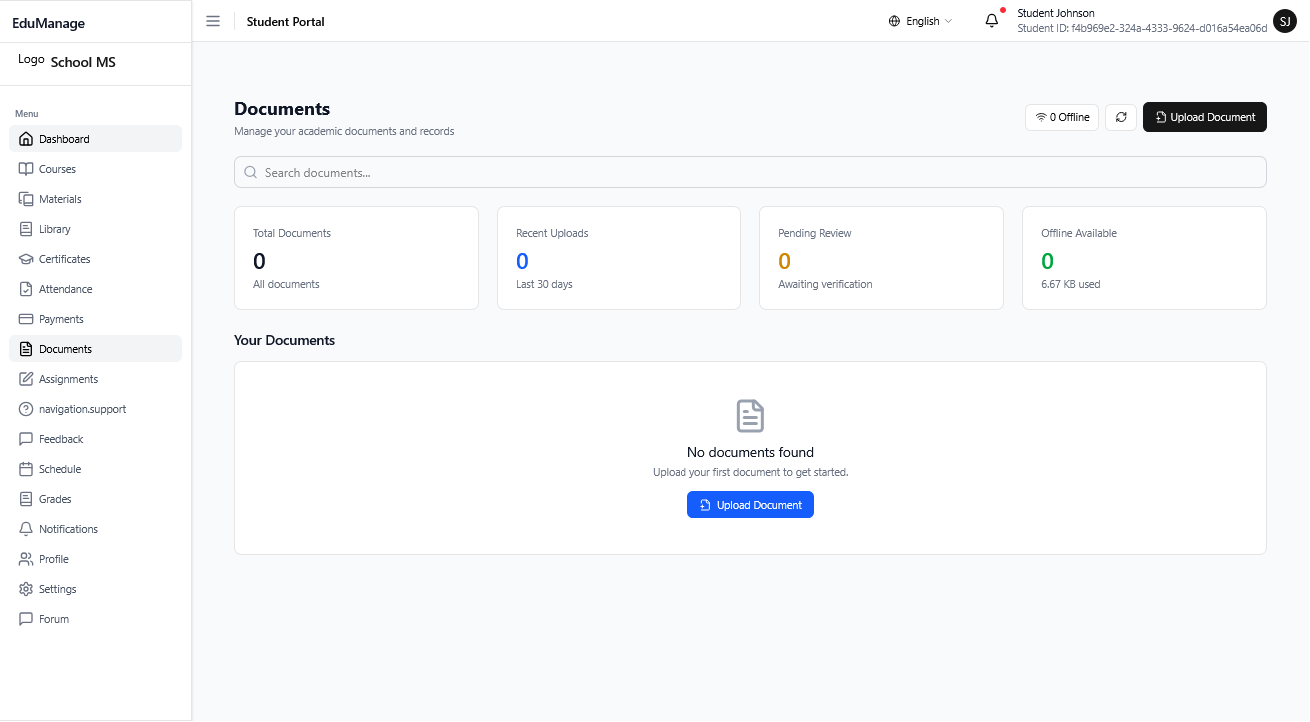
\includegraphics[width=\textwidth,height=0.55\textheight,keepaspectratio]{../pfe-pics/student/Screenshot 2025-06-09 at 22-46-22 Vite React TS.png}
            \caption{Assignment submission interface}
        \end{figure}
    \end{columns}
\end{frame}

\begin{frame}{Web Interface - Parent Portal}
    \begin{columns}
        \column{0.5\textwidth}
        \begin{figure}
            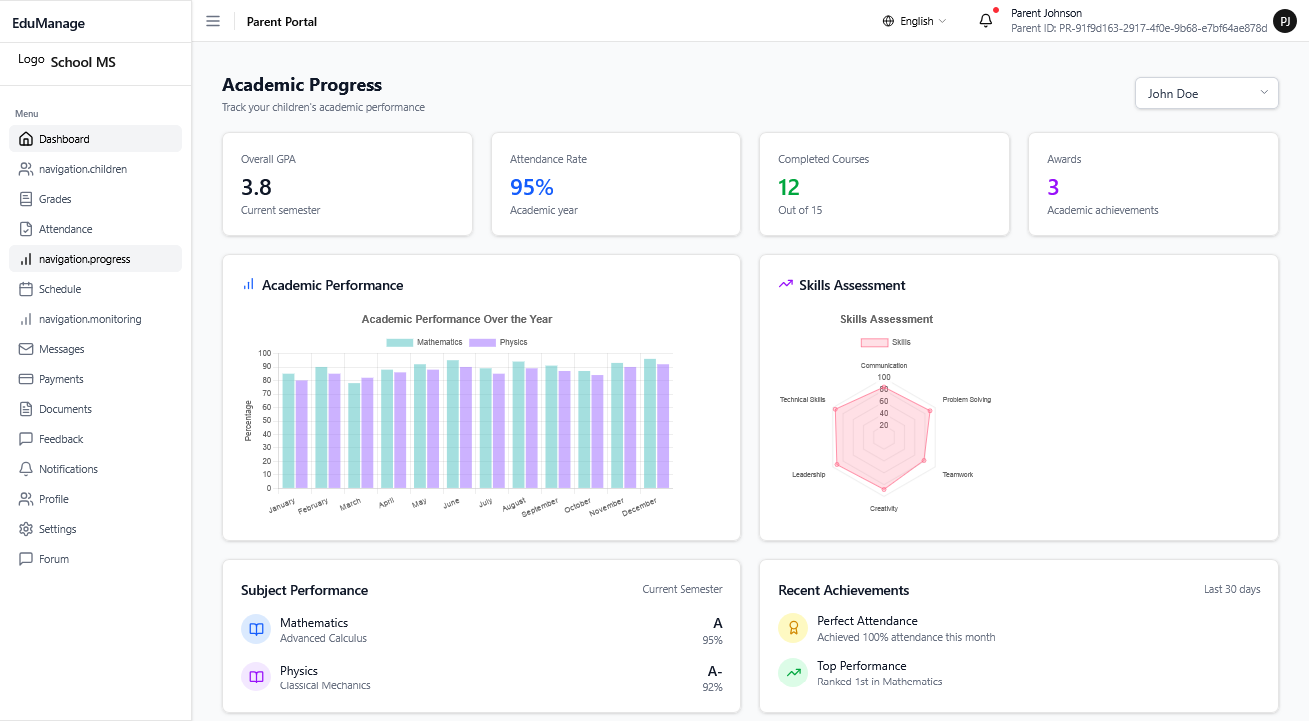
\includegraphics[width=\textwidth,height=0.55\textheight,keepaspectratio]{../pfe-pics/parent/Screenshot 2025-06-09 at 22-58-13 Vite React TS.png}
            \caption{Child progress monitoring}
        \end{figure}
        \column{0.5\textwidth}
        \begin{figure}
            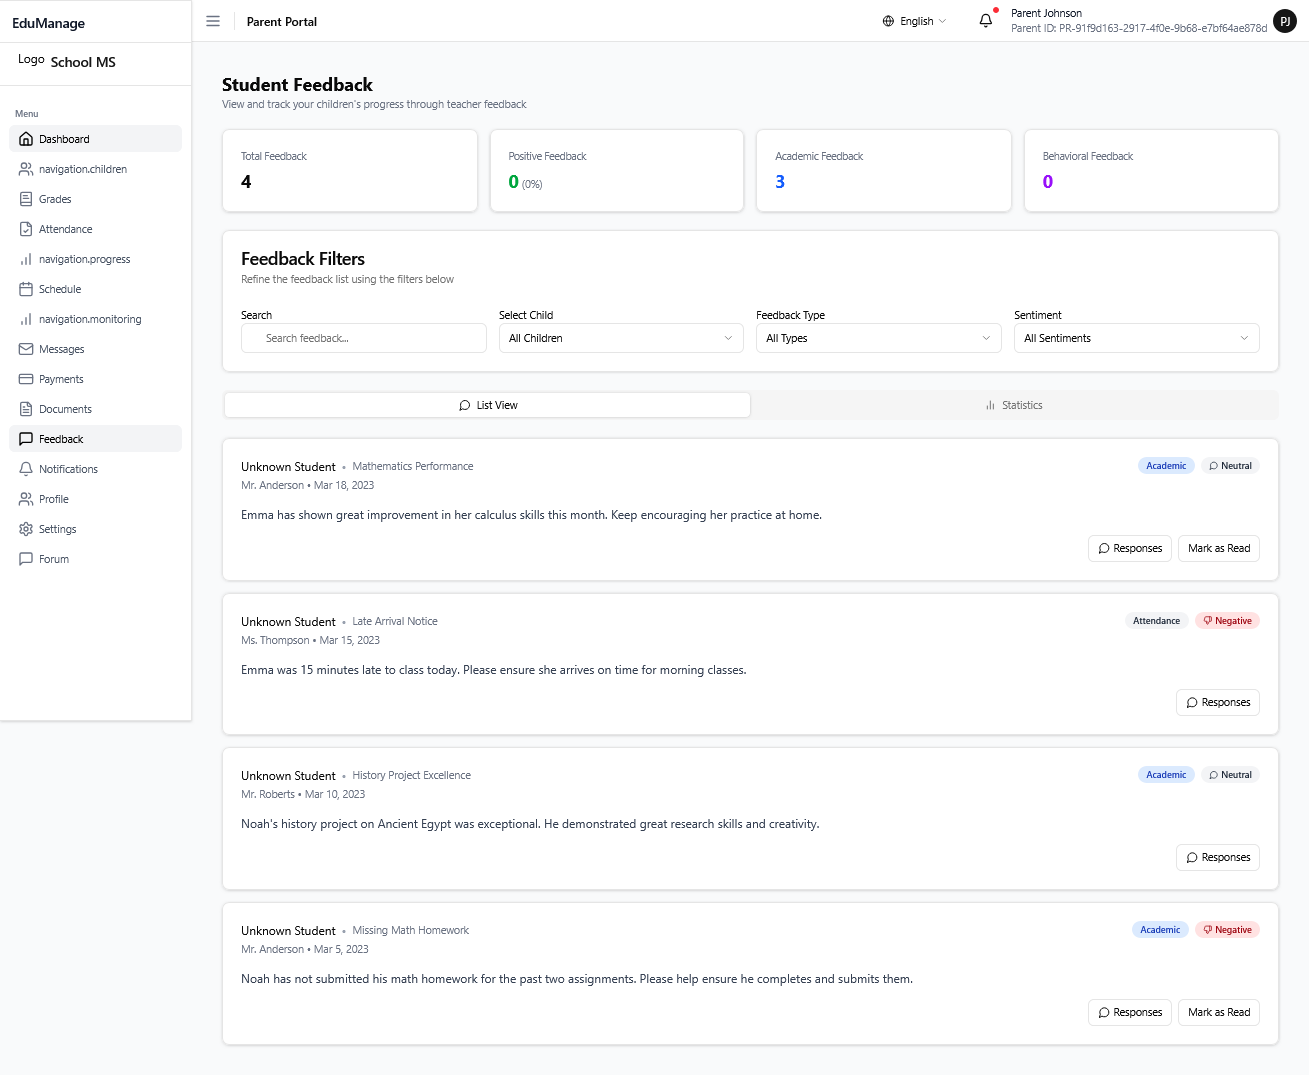
\includegraphics[width=\textwidth,height=0.55\textheight,keepaspectratio]{../pfe-pics/parent/Screenshot 2025-06-09 at 22-59-25 Vite React TS.png}
            \caption{Communication with teachers}
        \end{figure}
    \end{columns}
\end{frame}

\begin{frame}{Mobile Interface - Student App}
    \begin{columns}
        \column{0.33\textwidth}
        \begin{figure}
            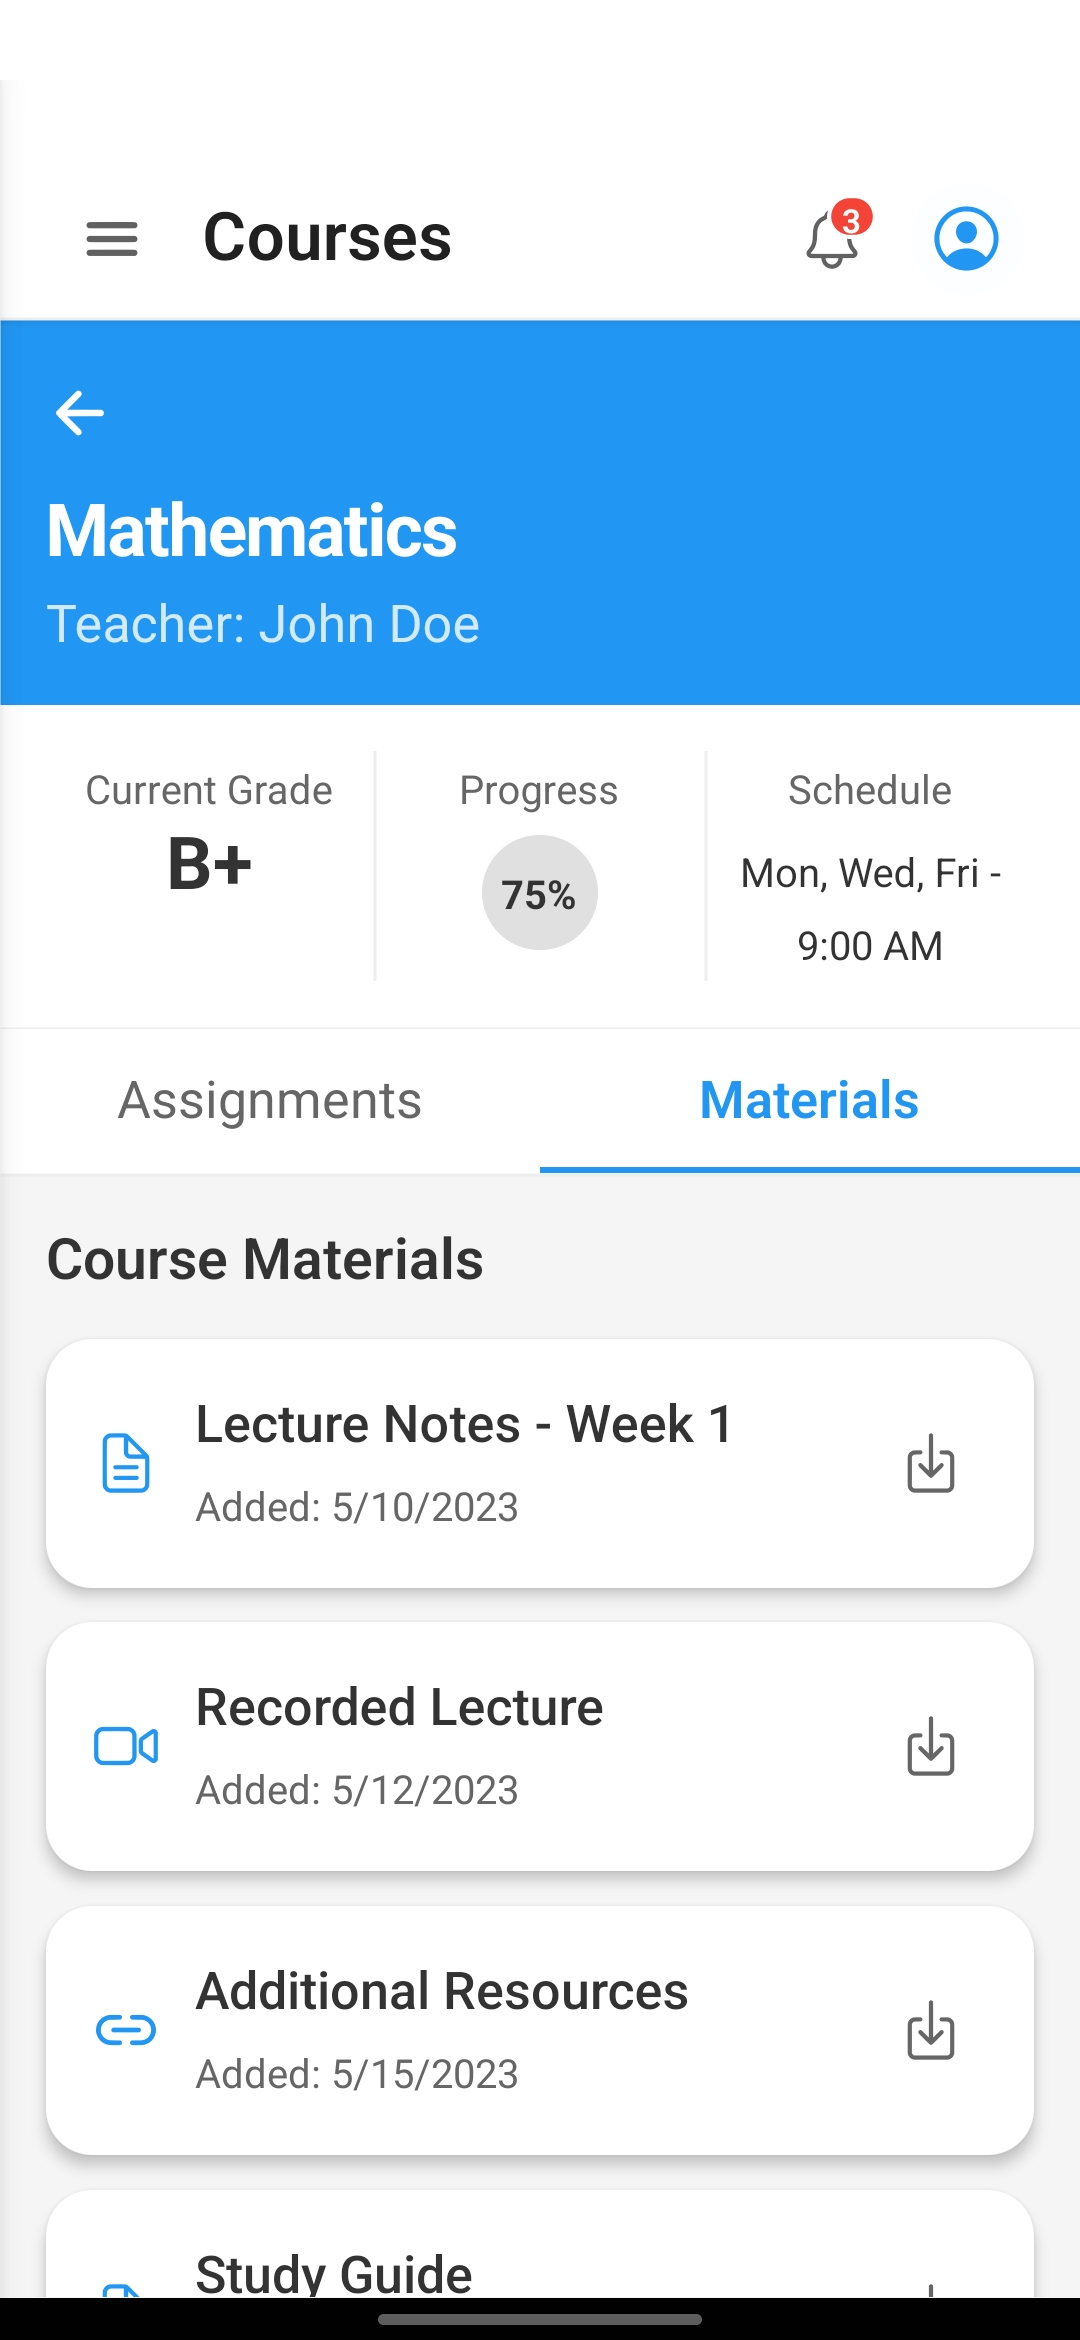
\includegraphics[width=\textwidth,height=0.6\textheight,keepaspectratio]{../pfe-pics/Mobile /Students/Screenshot_20250610_130150_Expo Go.jpg}
            \caption{Course details view}
        \end{figure}
        \column{0.33\textwidth}
        \begin{figure}
            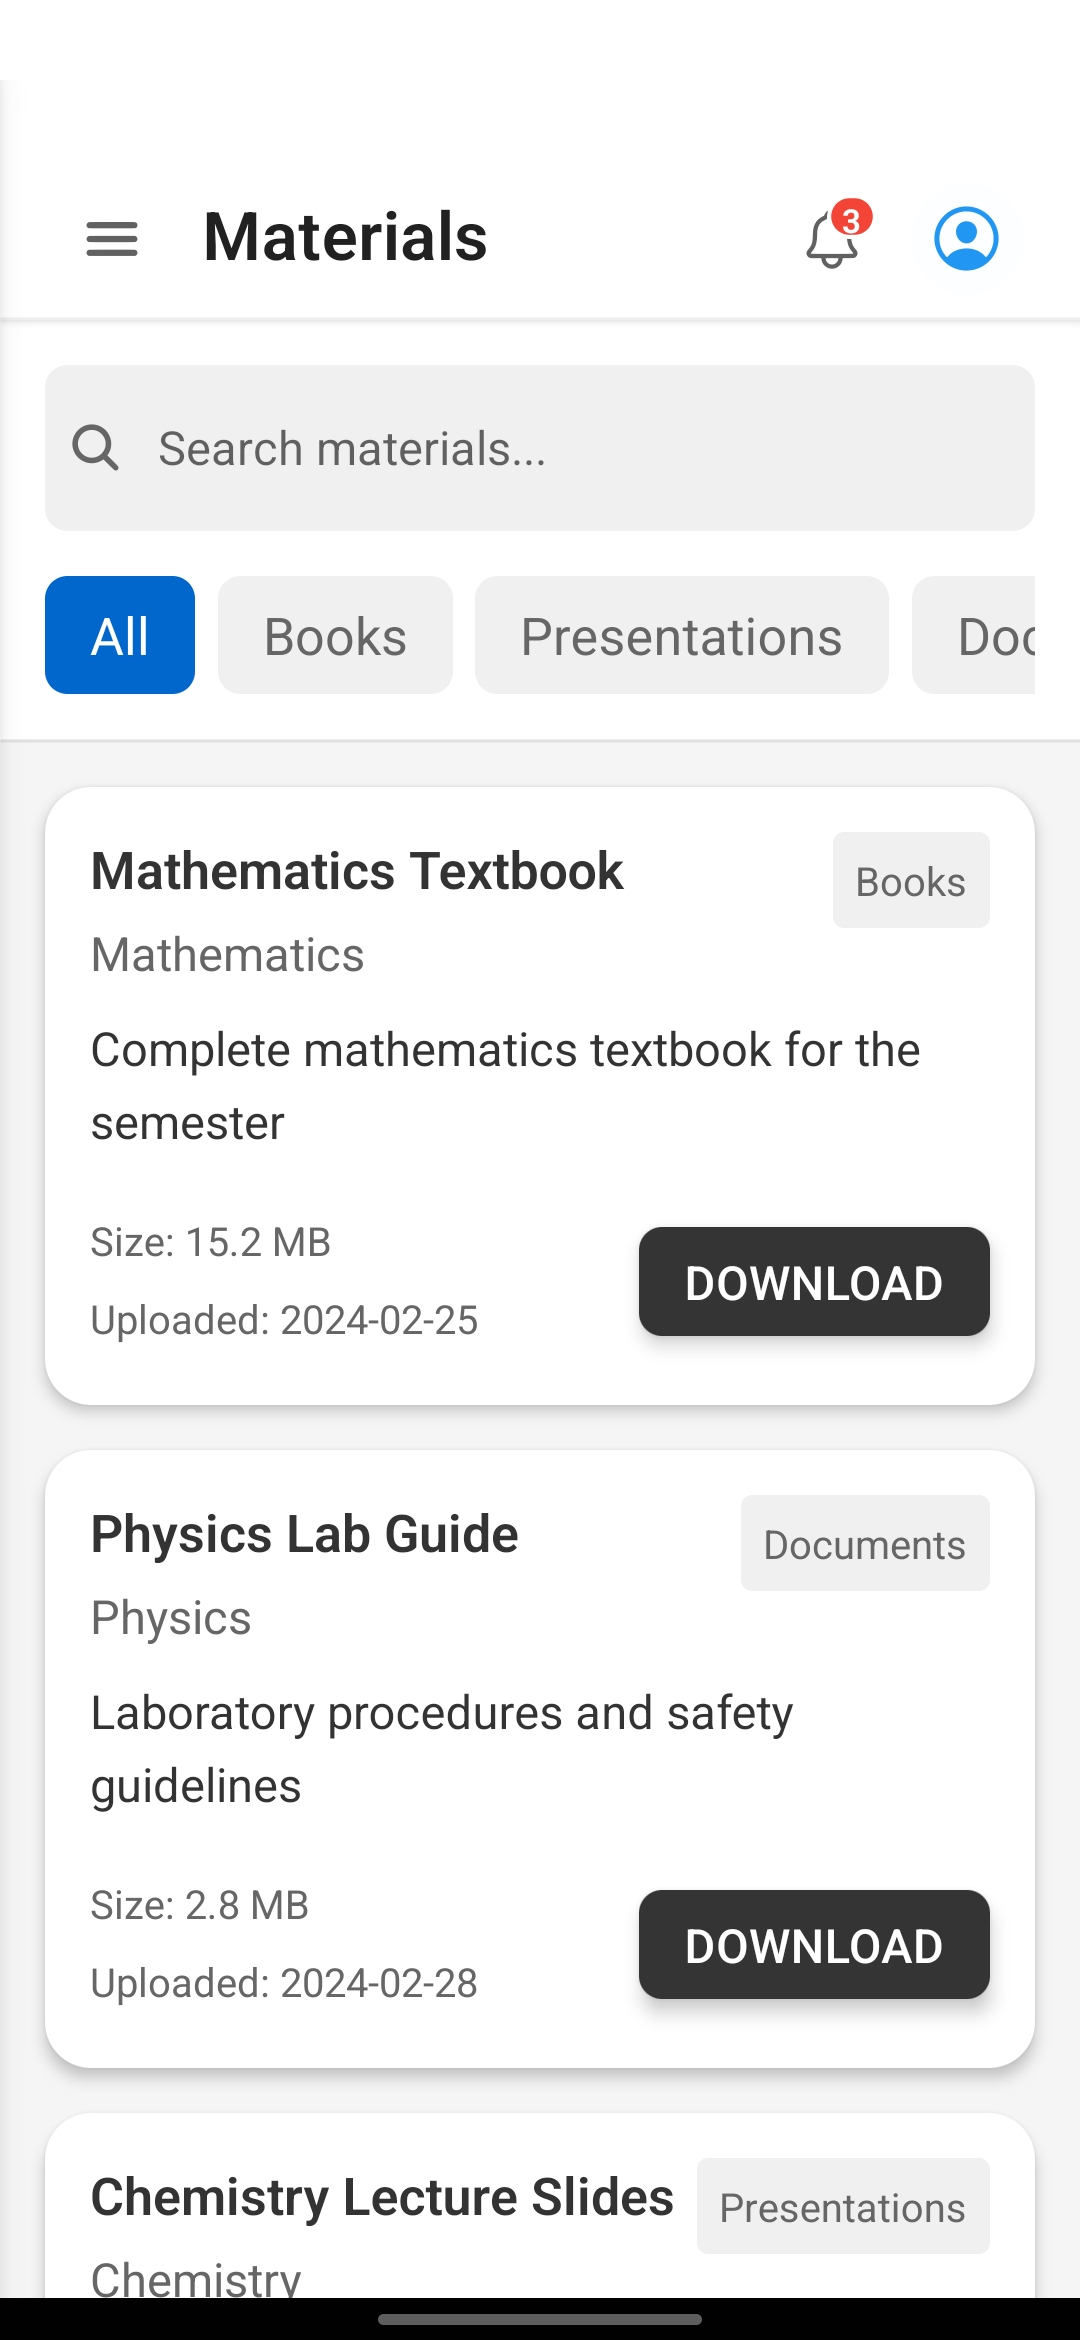
\includegraphics[width=\textwidth,height=0.6\textheight,keepaspectratio]{../pfe-pics/Mobile /Students/Screenshot_20250610_130310_Expo Go.jpg}
            \caption{Assignment management}
        \end{figure}
        \column{0.33\textwidth}
        \begin{figure}
            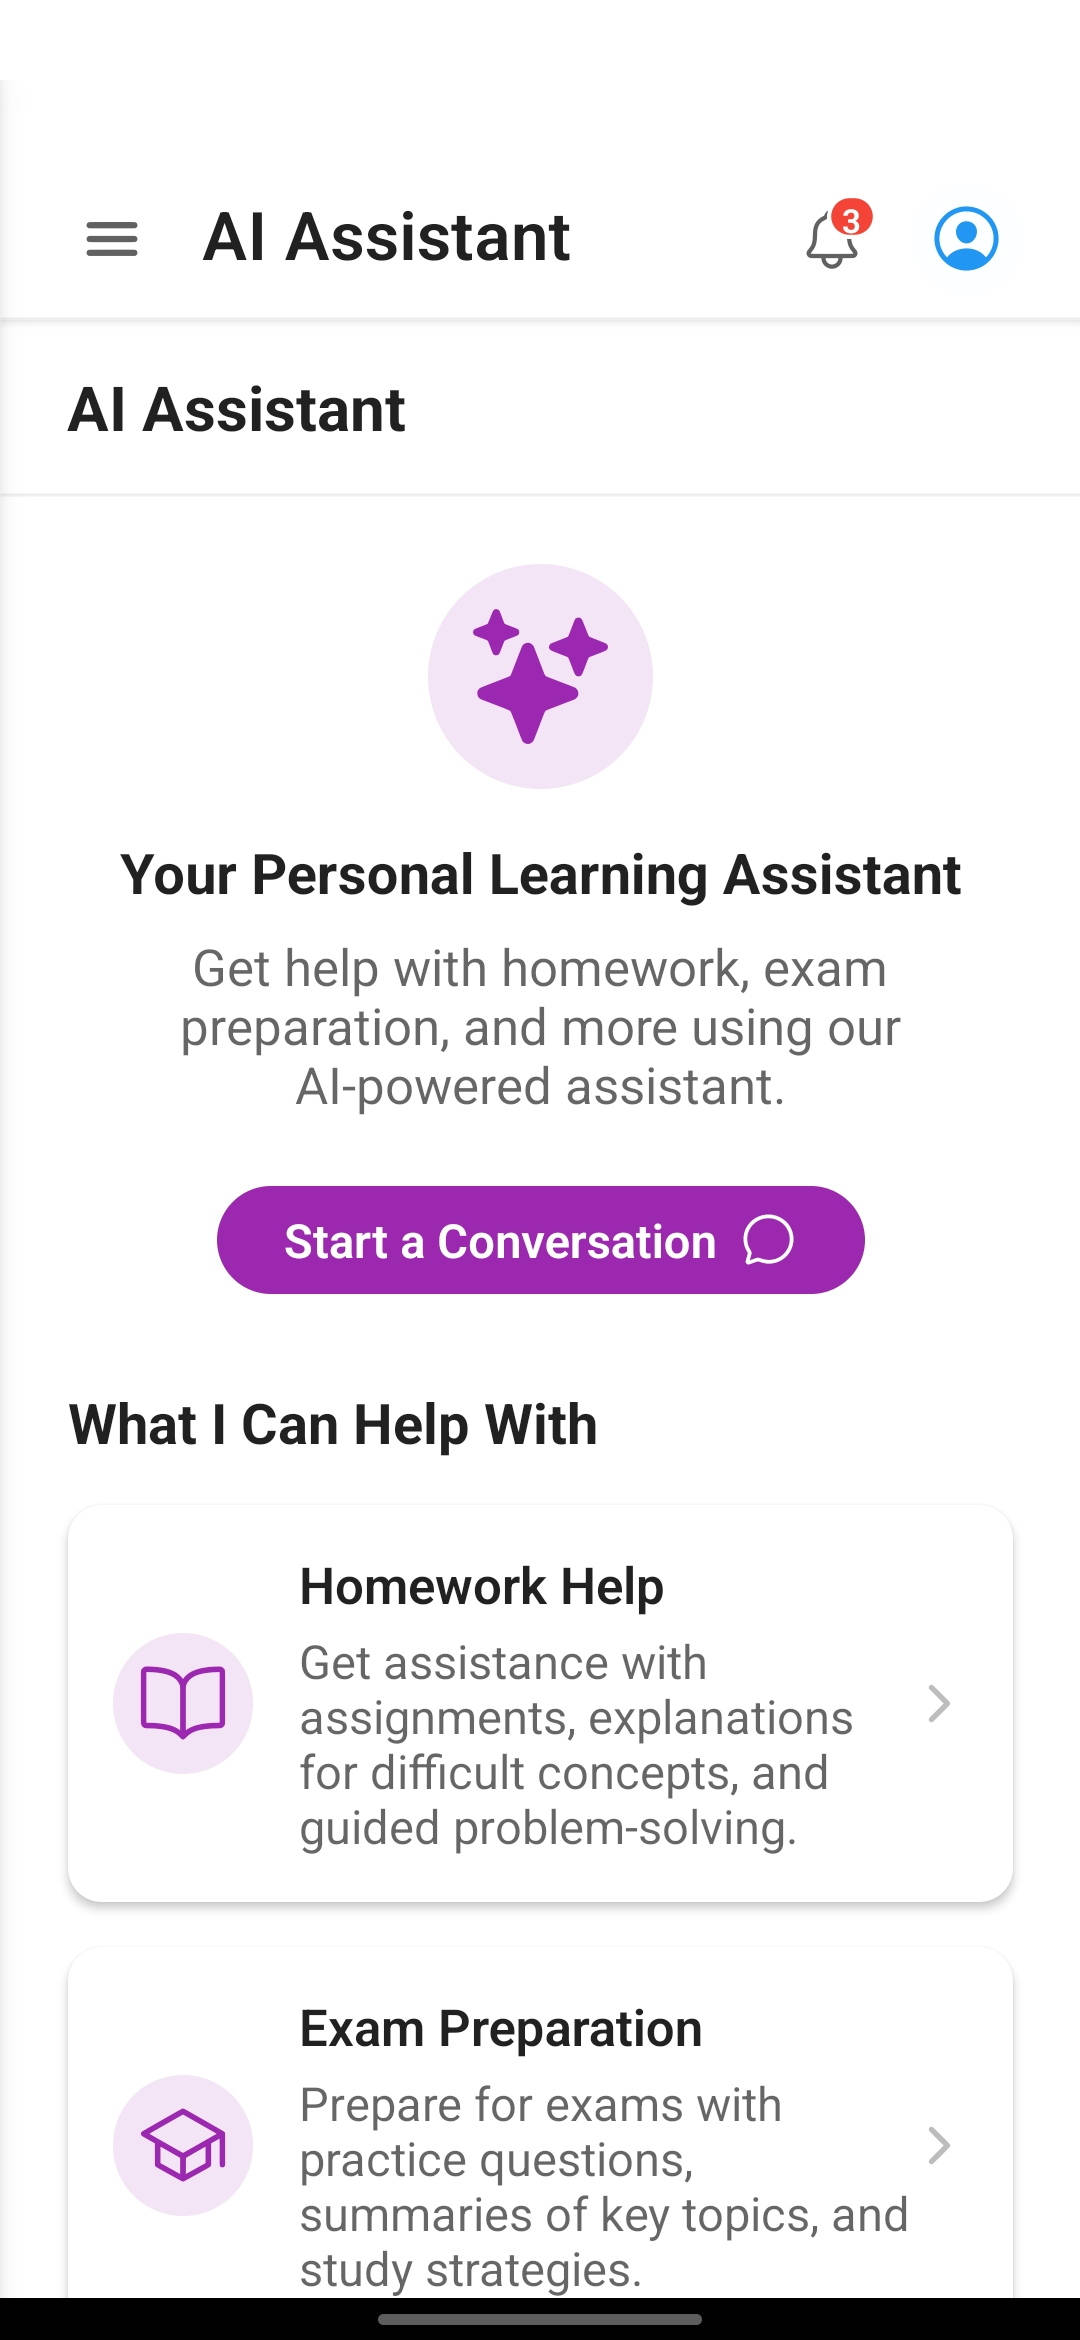
\includegraphics[width=\textwidth,height=0.6\textheight,keepaspectratio]{../pfe-pics/Mobile /Students/Screenshot_20250610_130351_Expo Go.jpg}
            \caption{Grade tracking interface}
        \end{figure}
    \end{columns}
\end{frame}

\begin{frame}{Mobile Interface - Teacher \& Parent Apps}
    \begin{columns}
        \column{0.5\textwidth}
        \begin{figure}
            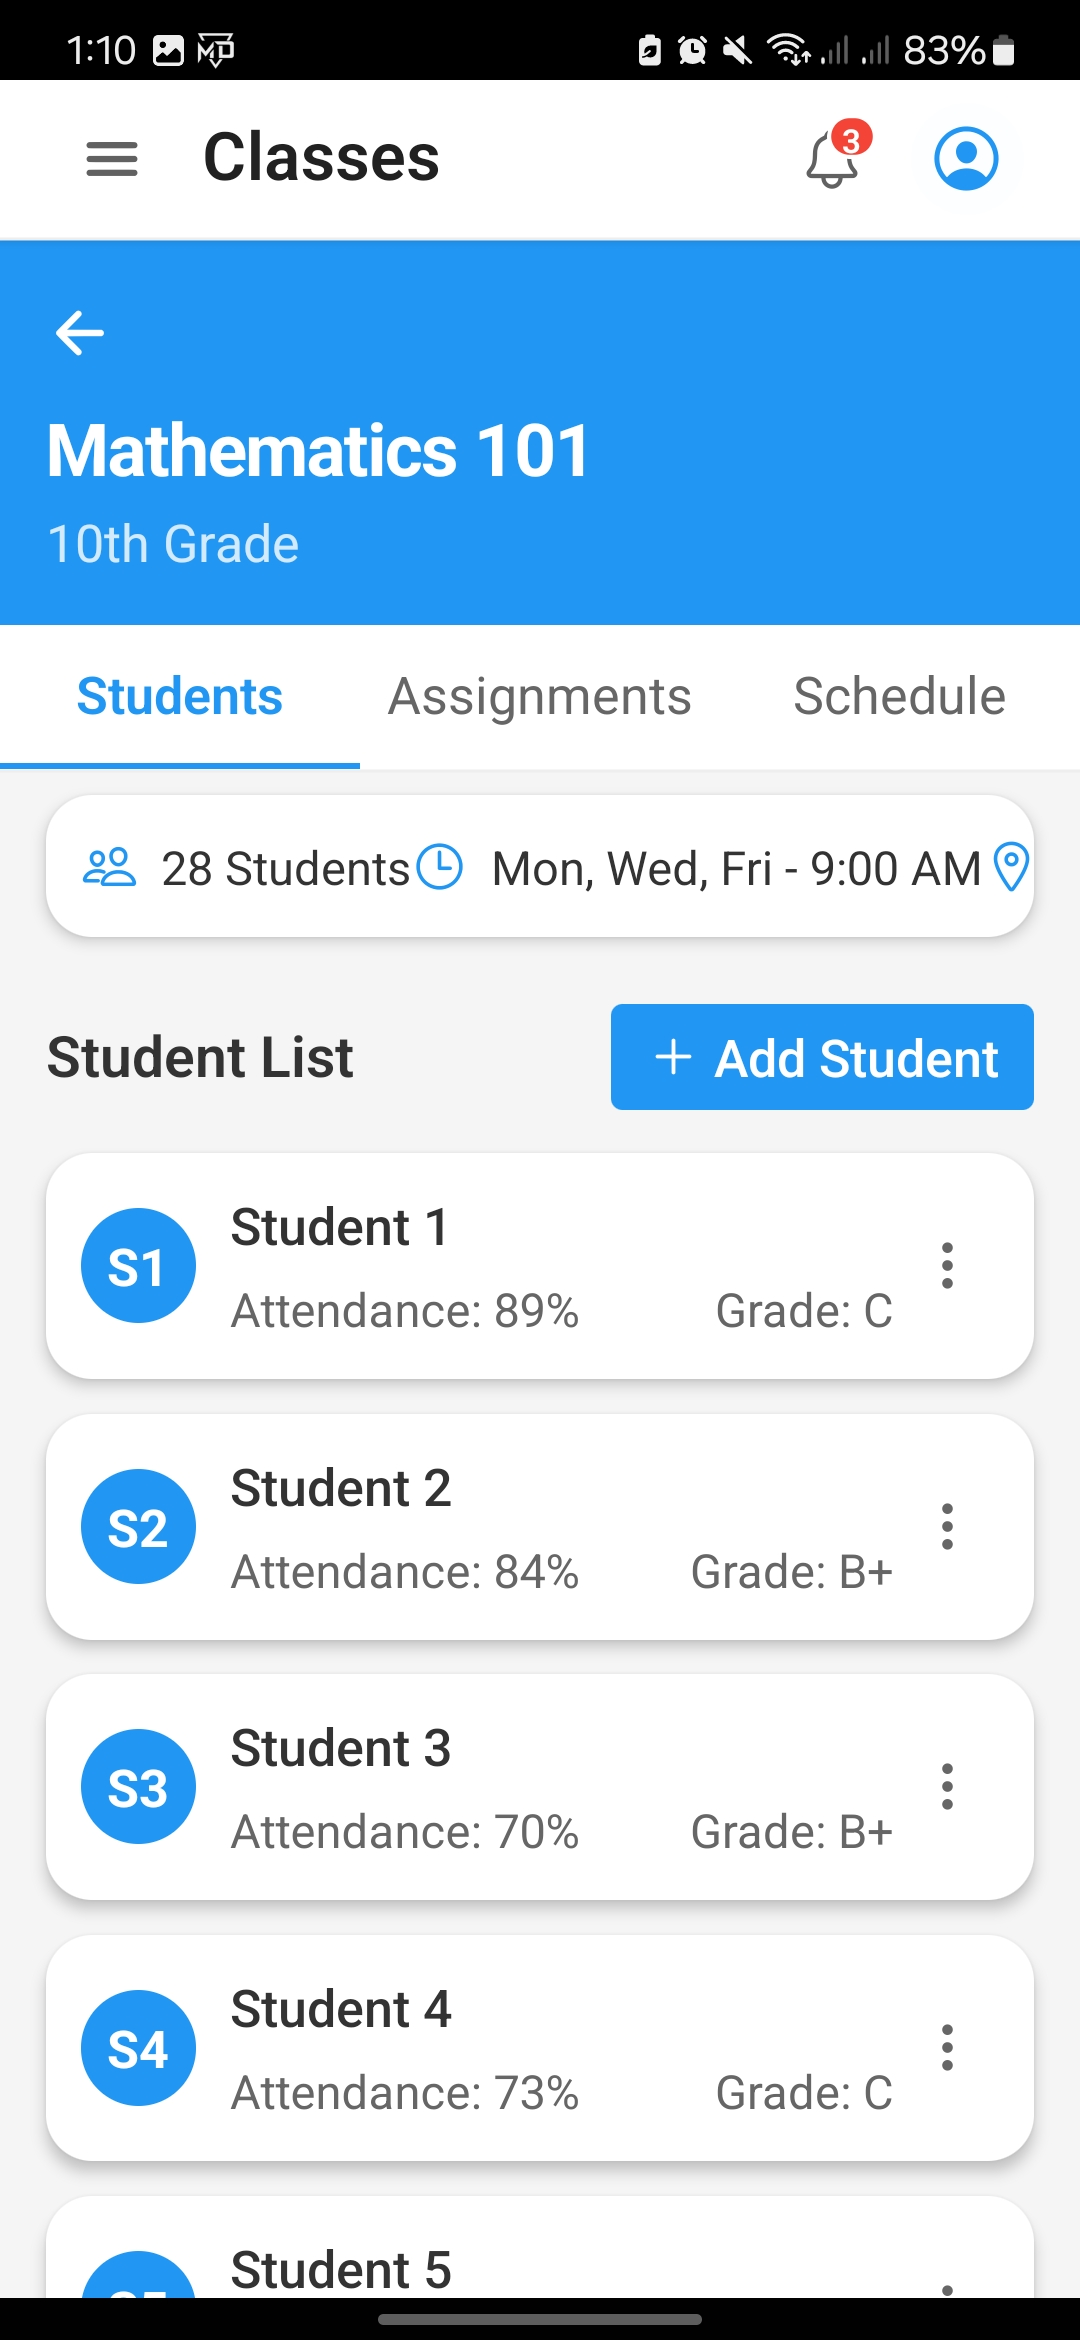
\includegraphics[width=0.7\textwidth,height=0.6\textheight,keepaspectratio]{../pfe-pics/Mobile /Teacher/Screenshot_20250610_131013_Expo Go.jpg}
            \caption{Teacher class management}
        \end{figure}
        \column{0.5\textwidth}
        \begin{figure}
            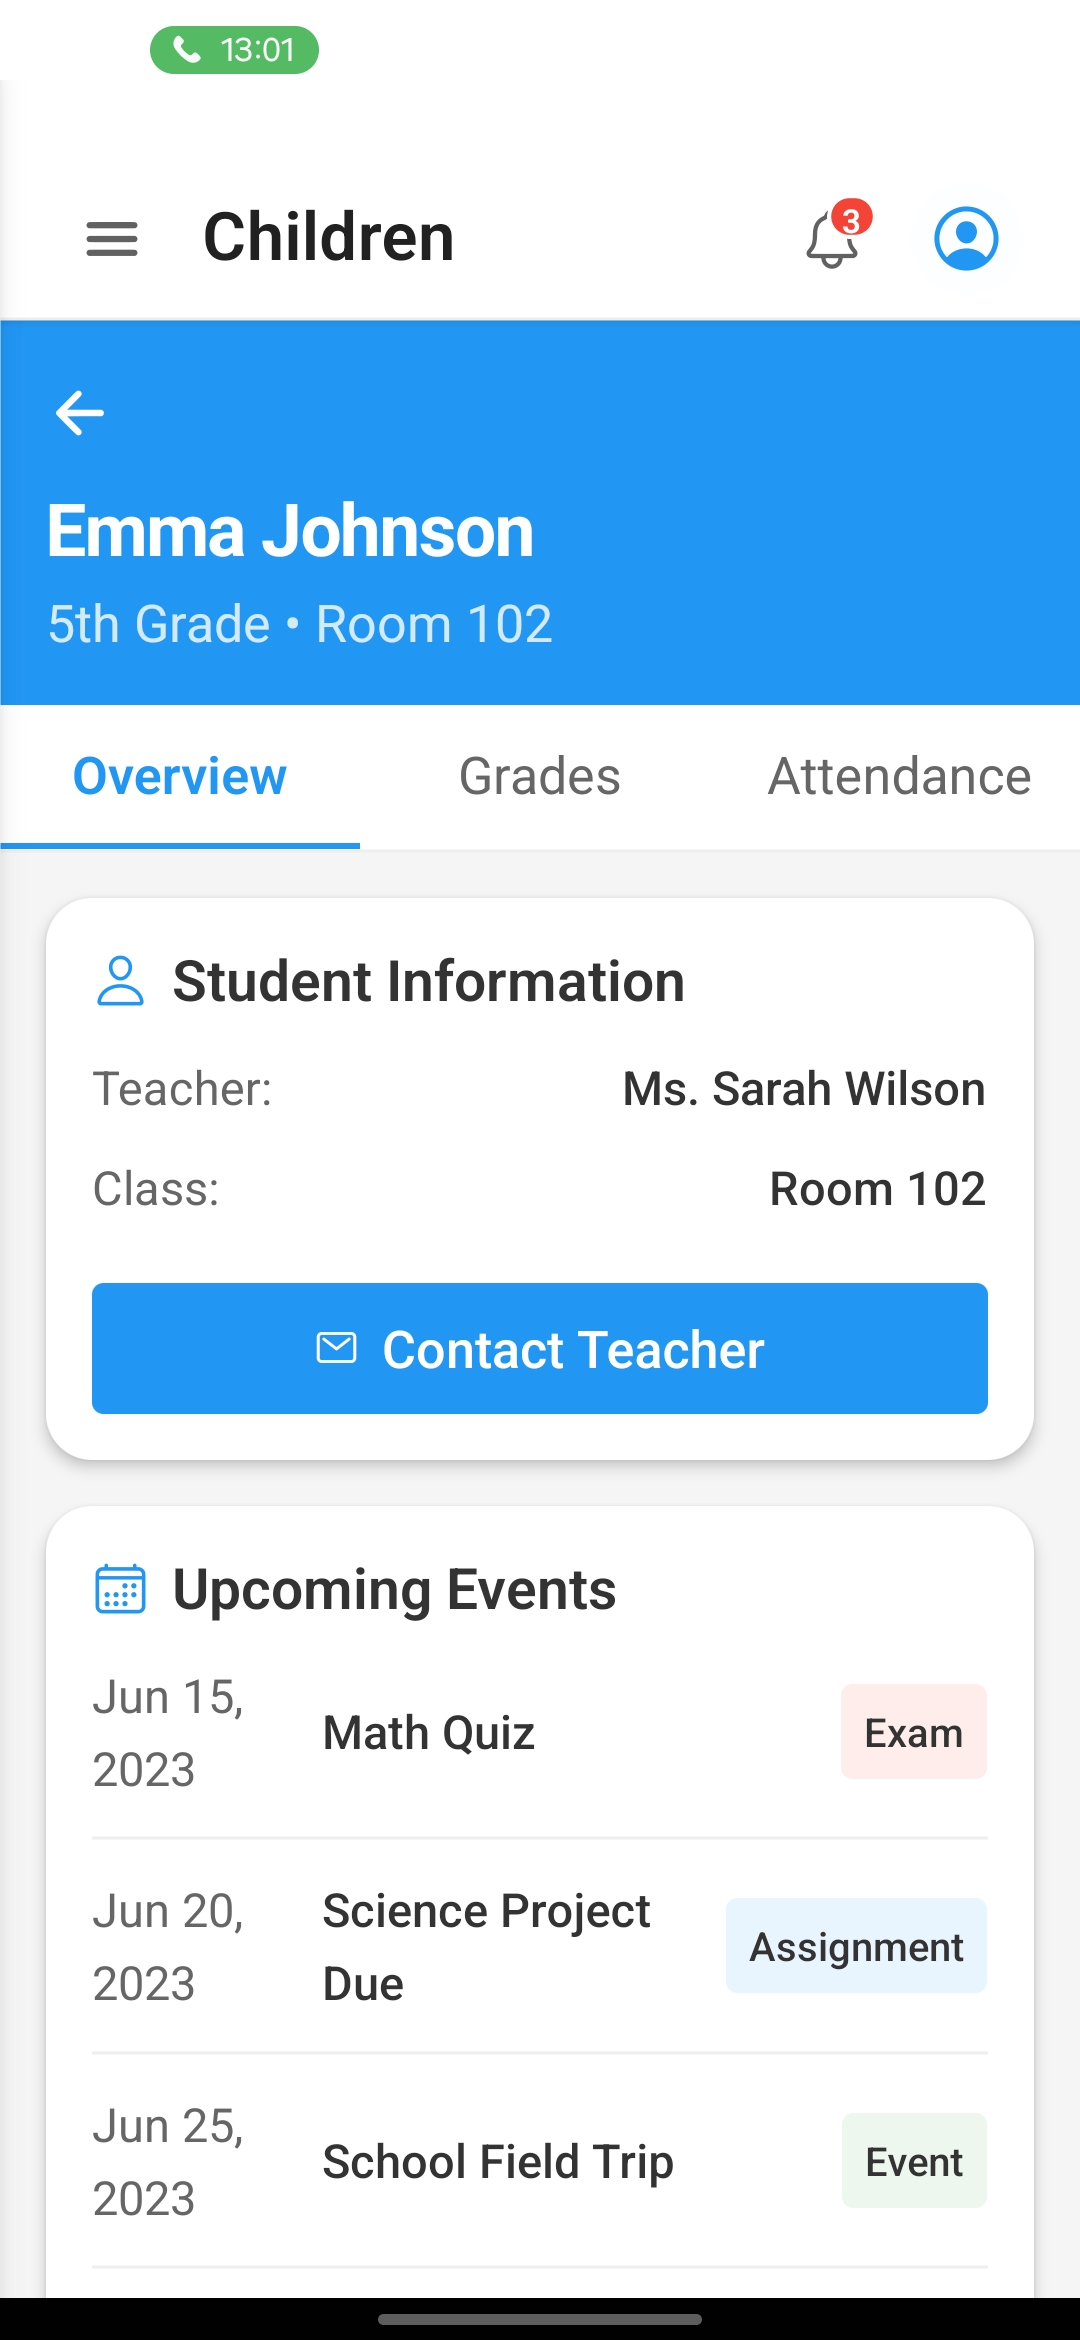
\includegraphics[width=0.7\textwidth,height=0.6\textheight,keepaspectratio]{../pfe-pics/Mobile /Parent /Screenshot_20250610_133032_Expo Go.jpg}
            \caption{Parent student monitoring}
        \end{figure}
    \end{columns}
\end{frame}

\begin{frame}{AI Profile Creation - Workflow}
    \begin{columns}
        \column{0.5\textwidth}
        \begin{figure}
            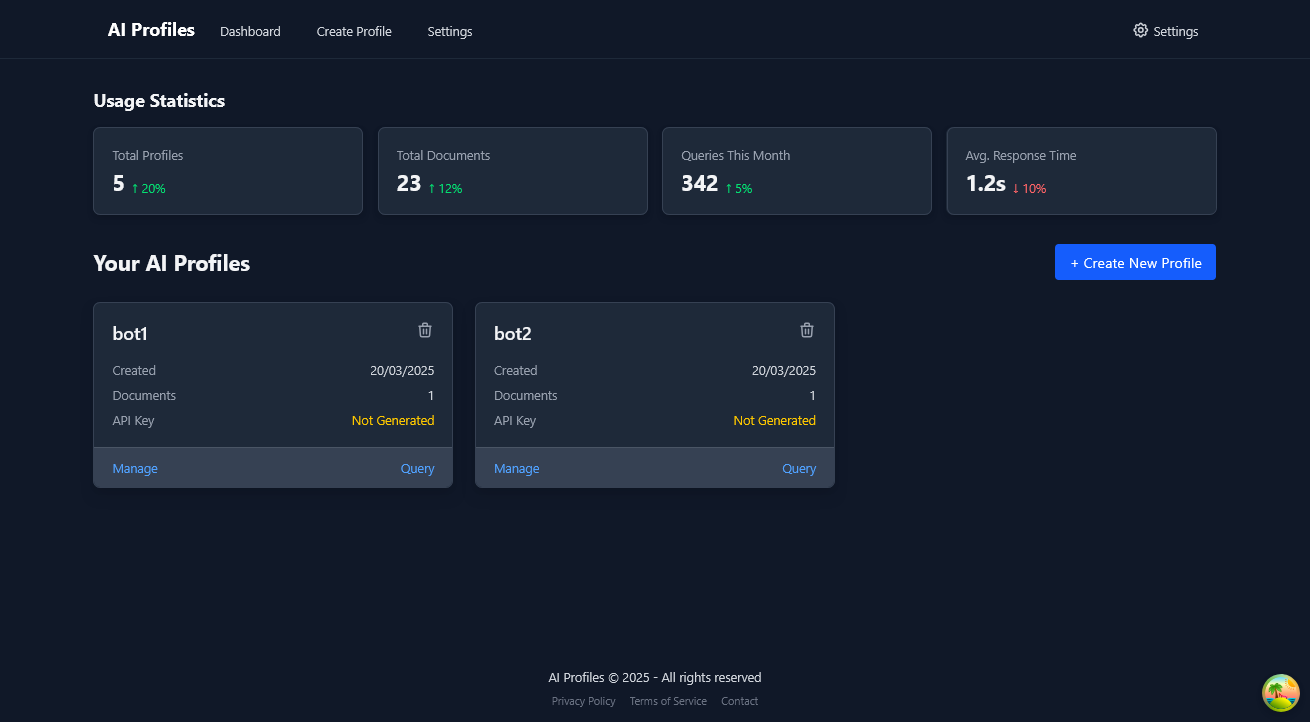
\includegraphics[width=\textwidth,height=0.55\textheight,keepaspectratio]{../pfe-pics/ai-profile-creation/dashboared_befor_adding_a_new_ai_profile.png}
            \caption{AI profiles dashboard}
        \end{figure}
        \column{0.5\textwidth}
        \begin{figure}
            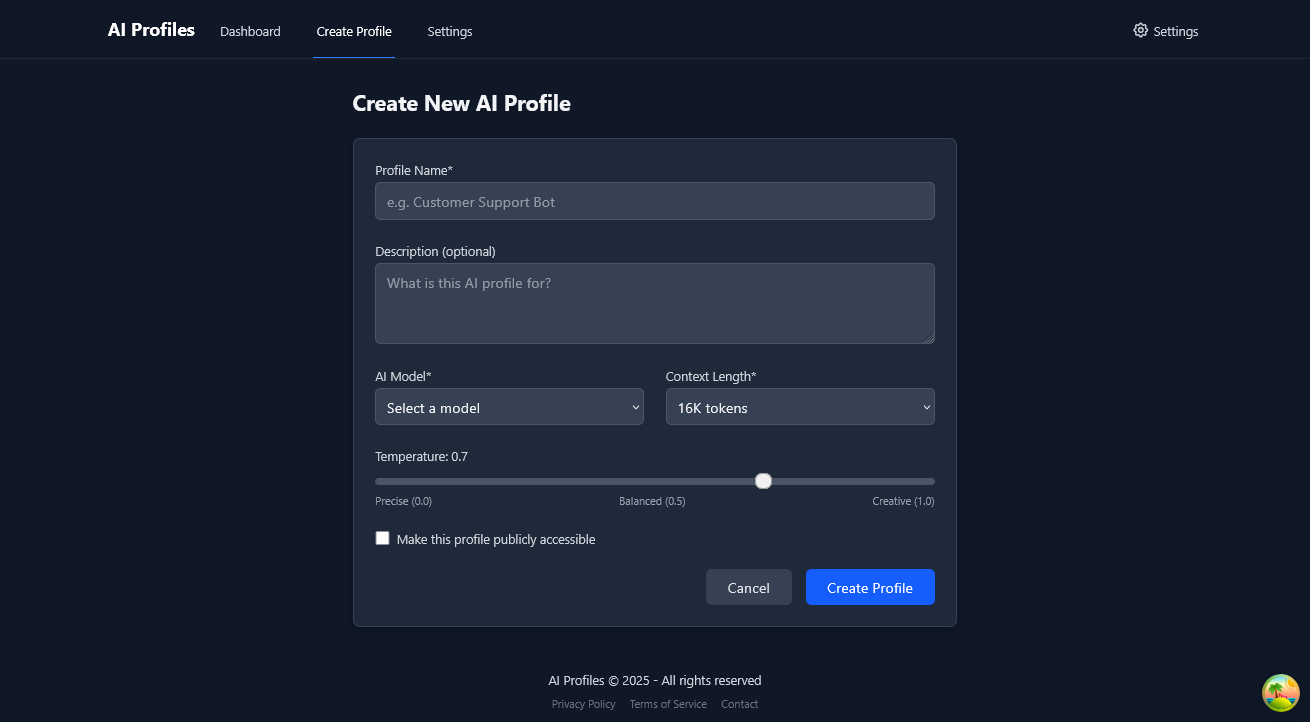
\includegraphics[width=\textwidth,height=0.55\textheight,keepaspectratio]{../pfe-pics/ai-profile-creation/creating_and_ai_prifile.png}
            \caption{Profile creation interface}
        \end{figure}
    \end{columns}
\end{frame}

\begin{frame}{AI Profile Creation - Document Processing}
    \begin{columns}
        \column{0.5\textwidth}
        \begin{figure}
            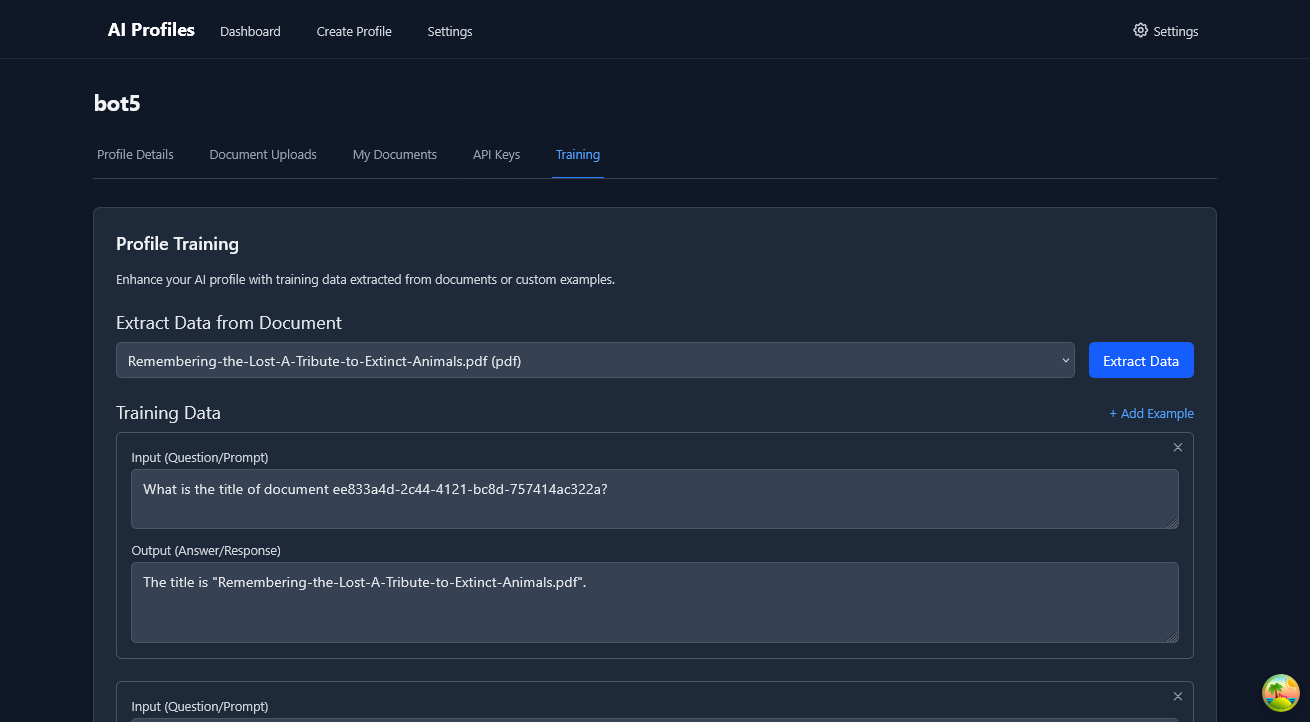
\includegraphics[width=\textwidth,height=0.55\textheight,keepaspectratio]{../pfe-pics/ai-profile-creation/extract_info_from_file_and_training_pfrile.png}
            \caption{Document upload and extraction}
        \end{figure}
        \column{0.5\textwidth}
        \begin{figure}
            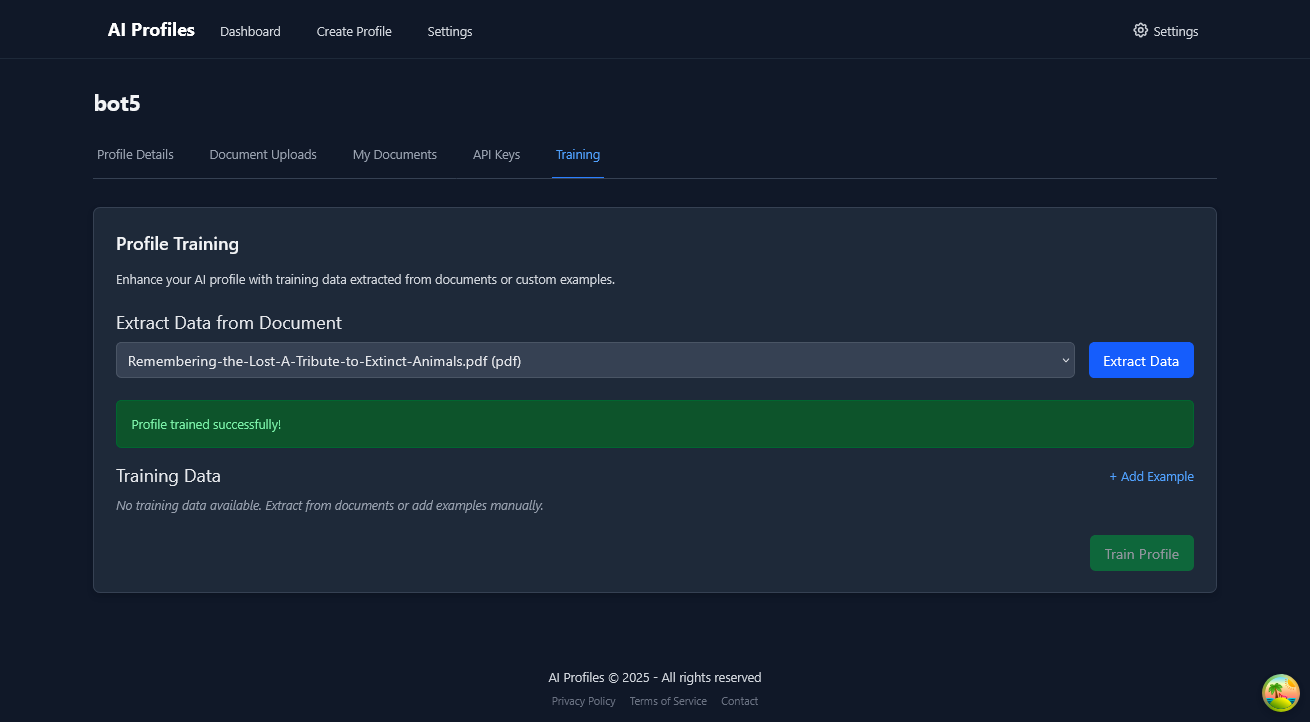
\includegraphics[width=\textwidth,height=0.55\textheight,keepaspectratio]{../pfe-pics/ai-profile-creation/succesful_knoladge_integration.png}
            \caption{Successful knowledge integration}
        \end{figure}
    \end{columns}
\end{frame}

\begin{frame}{AI Profile - Usage \& Integration}
    \begin{columns}
        \column{0.5\textwidth}
        \begin{figure}
            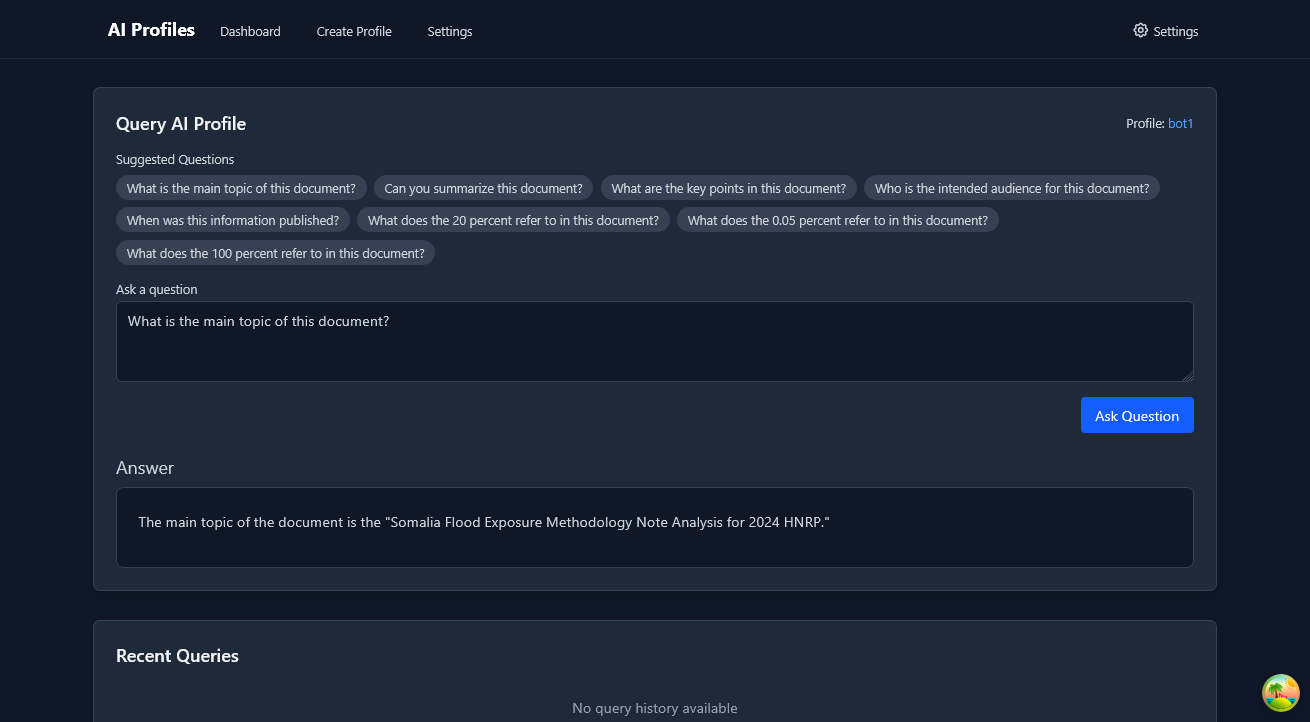
\includegraphics[width=\textwidth,height=0.55\textheight,keepaspectratio]{../pfe-pics/ai-profile-creation/chat_interface_to_test_the_profile.png}
            \caption{Conversational testing interface}
        \end{figure}
        \column{0.5\textwidth}
        \begin{figure}
            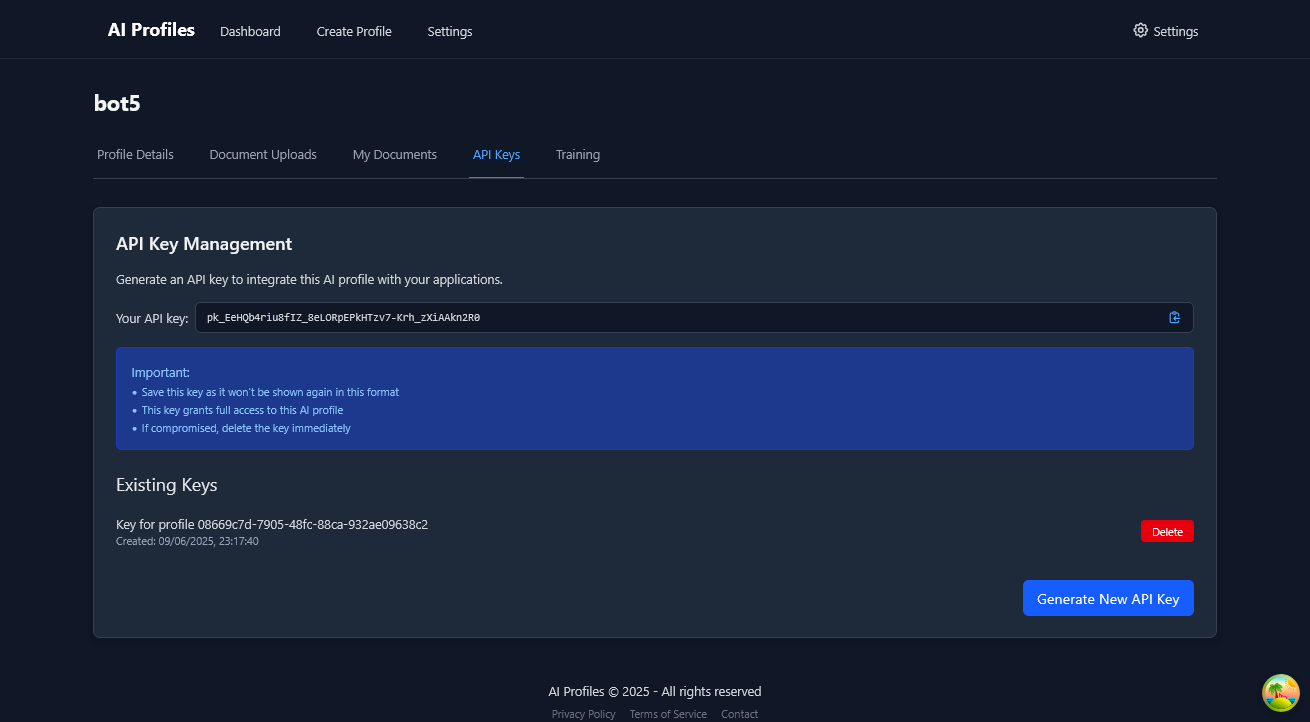
\includegraphics[width=\textwidth,height=0.55\textheight,keepaspectratio]{../pfe-pics/ai-profile-creation/create_and_api_key_for_trained_profile.png}
            \caption{API key generation for integration}
        \end{figure}
    \end{columns}
\end{frame}

\section{Implementation}

\begin{frame}{Technology Stack}
    \begin{columns}
        \column{0.5\textwidth}
        \textbf{School Management System:}
        \begin{itemize}
            \item \textbf{Frontend:} React, React Native, Tailwind CSS
            \item \textbf{Backend:} Node.js, Express
            \item \textbf{Database:} MongoDB
            \item \textbf{Authentication:} JWT
            \item \textbf{Deployment:} Docker, AWS
        \end{itemize}
        \column{0.5\textwidth}
        \textbf{AI Profiles Creation:}
        \begin{itemize}
            \item \textbf{Frontend:} React, TypeScript
            \item \textbf{Backend:} FastAPI (Python)
            \item \textbf{Database:} PostgreSQL
            \item \textbf{AI Integration:} OpenRouter API
            \item \textbf{Vector Store:} Pinecone
        \end{itemize}
    \end{columns}
\end{frame}

\begin{frame}{Development Approach}
    \begin{itemize}
        \item \textbf{Hybrid Agile Methodology}
        \begin{itemize}
            \item Iterative development
            \item Regular review sessions
            \item Adaptation to user feedback
        \end{itemize}
        \vspace{0.3cm}
        \item \textbf{Project Timeline (Dec 2024 - May 2025)}
        \begin{itemize}
            \item Initial Phase: Requirements analysis, design
            \item Development Phase 1: School Management System
            \item Development Phase 2: AI Profiles Creation (partially completed)
            \item Project suspended in April 2025 due to national exams
        \end{itemize}
    \end{itemize}
\end{frame}

\begin{frame}{Project Timeline}
    \begin{figure}
        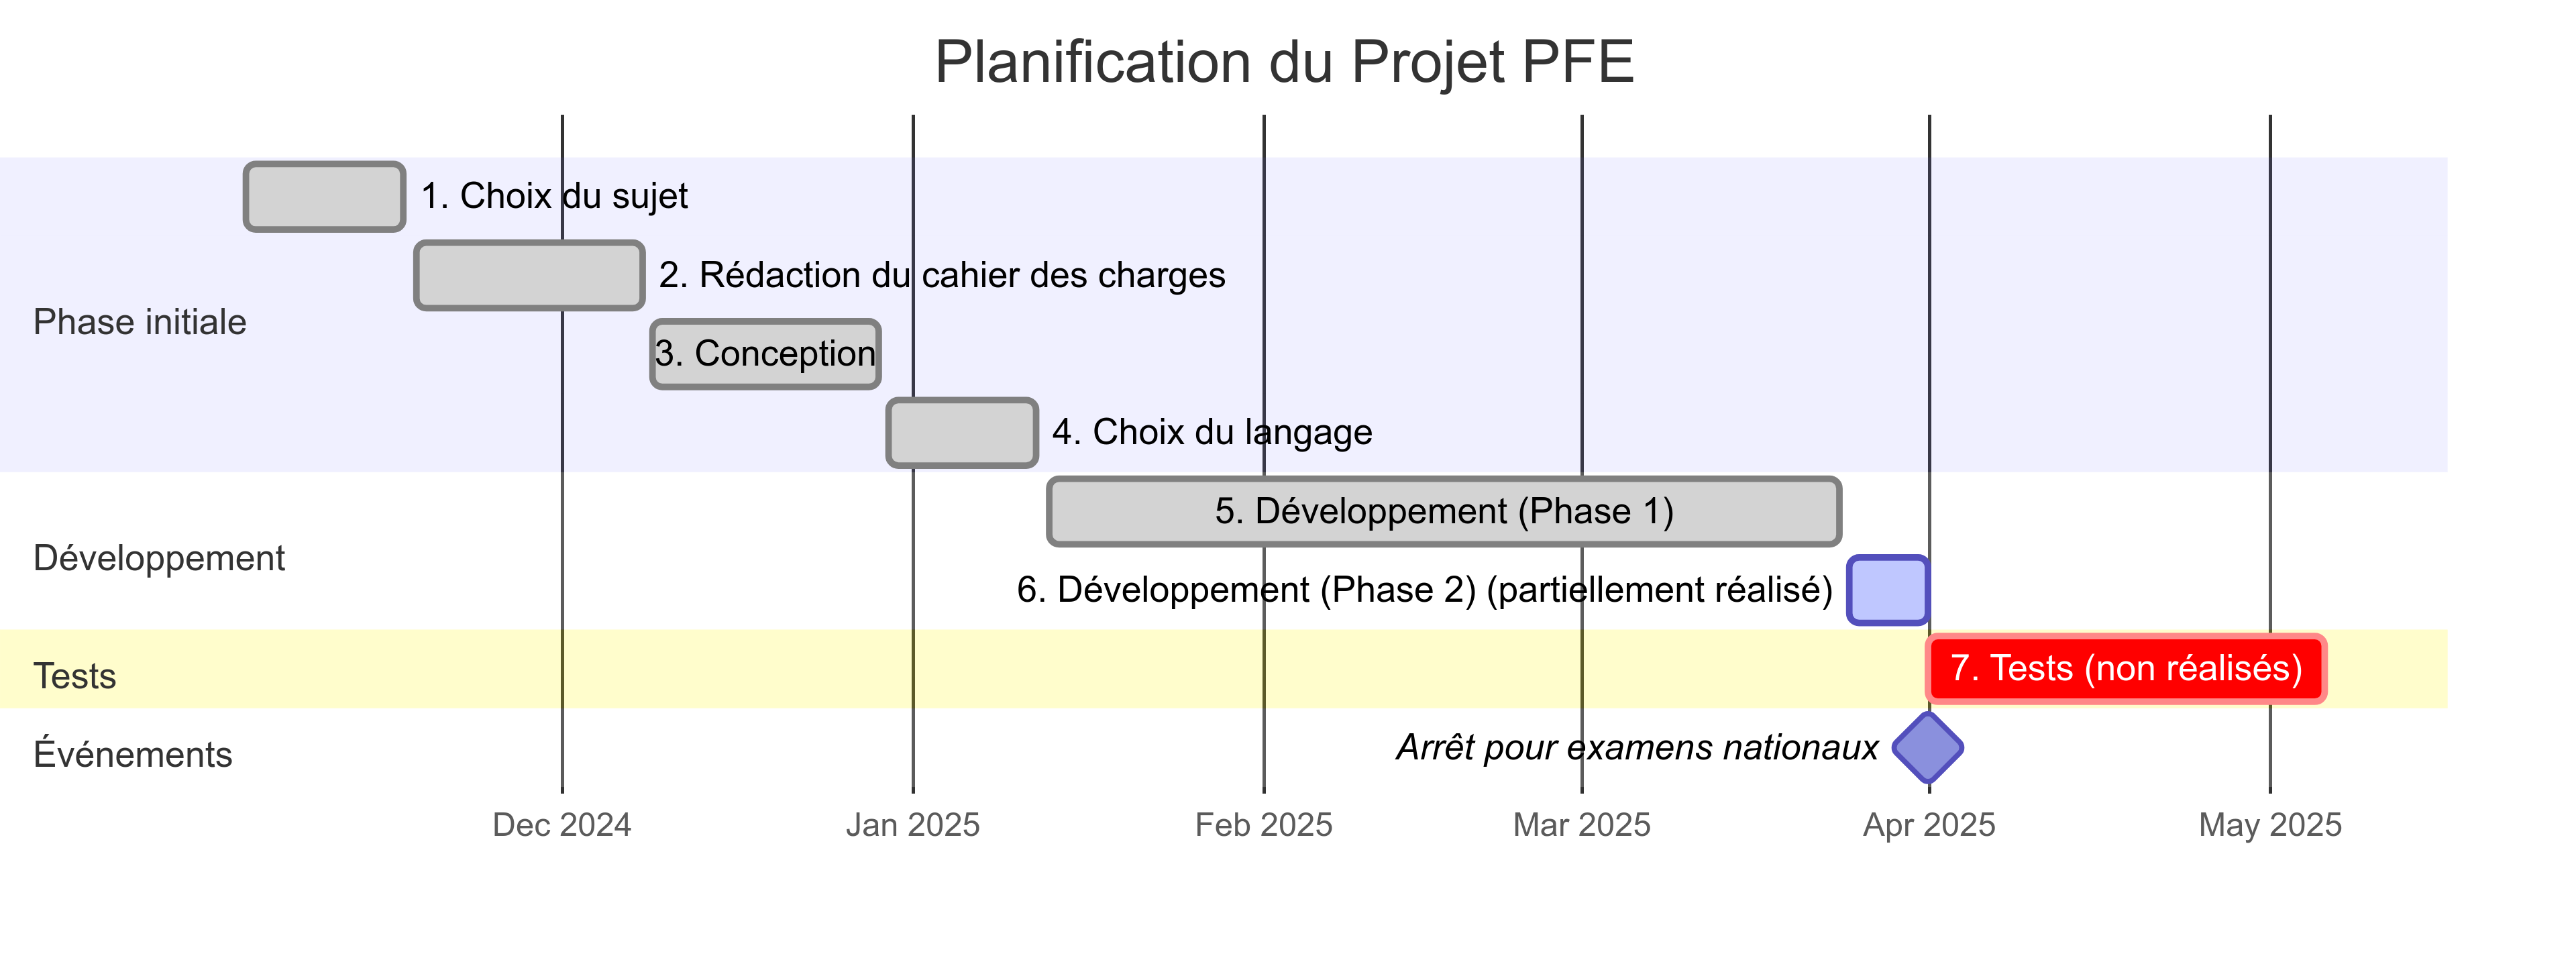
\includegraphics[width=0.9\textwidth,height=0.7\textheight,keepaspectratio]{../pfe-pics/diagrames/Mermaid Chart - Create complex, visual diagrams with text. A smarter way of creating diagrams.-2025-06-10-203842.png}
        \caption{Project Gantt Chart}
    \end{figure}
\end{frame}

\begin{frame}{Critical Path Analysis}
    \begin{figure}
        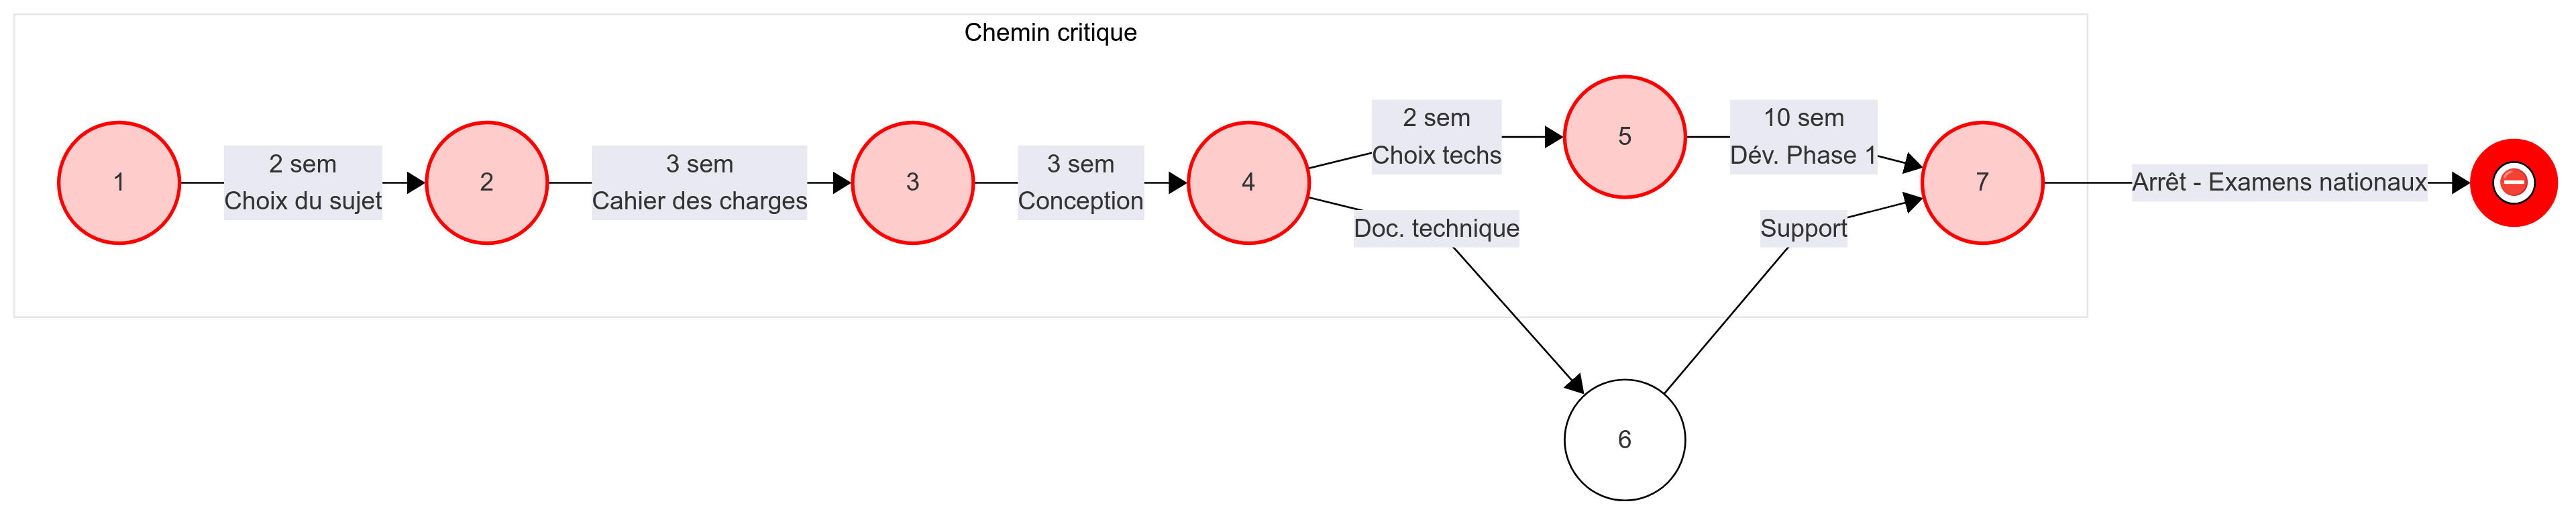
\includegraphics[width=0.9\textwidth,height=0.7\textheight,keepaspectratio]{../pfe-pics/diagrames/Mermaid Chart - Create complex, visual diagrams with text. A smarter way of creating diagrams.-2025-06-10-203658.png}
        \caption{Project Critical Path Analysis}
    \end{figure}
\end{frame}

\section{Challenges and Solutions}

\begin{frame}{Technical Challenges}
    \begin{columns}
        \column{0.5\textwidth}
        \textbf{School Management System:}
        \begin{itemize}
            \item User role permissions complexity
            \item Mobile-web code sharing
            \item Real-time notifications
            \item Data consistency across platforms
        \end{itemize}
        \column{0.5\textwidth}
        \textbf{AI Profiles Creation:}
        \begin{itemize}
            \item Document processing optimization
            \item Context preservation in chunking
            \item Embedding model selection
            \item Response quality management
        \end{itemize}
    \end{columns}
    \vspace{0.5cm}
    \textbf{Solutions:}
    \begin{itemize}
        \item Component-based architecture for reusability
        \item Progressive enhancement for feature deployment
        \item Optimization through caching and asynchronous processing
    \end{itemize}
\end{frame}

\section{Future Development}

\begin{frame}{Future Enhancements}
    \begin{columns}
        \column{0.5\textwidth}
        \textbf{School Management System:}
        \begin{itemize}
            \item Advanced analytics dashboard
            \item Integration with learning platforms
            \item Automated scheduling system
            \item Enhanced reporting tools
            \item Offline functionality improvements
        \end{itemize}
        \column{0.5\textwidth}
        \textbf{AI Profiles Creation:}
        \begin{itemize}
            \item Fine-tuning capabilities
            \item Multi-modal content support
            \item Collaborative profile editing
            \item Performance optimizations
            \item Enhanced security features
        \end{itemize}
    \end{columns}
\end{frame}

\begin{frame}{Conclusion}
    \begin{itemize}
        \item \textbf{Achievements:}
        \begin{itemize}
            \item Successful implementation of School Management System
            \item Functional AI Profiles Creation prototype
            \item Integration between both systems
            \item User-friendly interfaces across platforms
        \end{itemize}
        \vspace{0.5cm}
        \item \textbf{Lessons Learned:}
        \begin{itemize}
            \item Importance of modular architecture
            \item Value of continuous testing
            \item Challenge of integrating AI systems
            \item Need for adaptive project planning
        \end{itemize}
    \end{itemize}
\end{frame}

\begin{frame}
    \begin{center}
        \Huge Thank You
        \vspace{1cm}
        
        \Large Questions?
    \end{center}
\end{frame}

\end{document} 